\documentclass[UTF8,a4paper]{article}
\usepackage{fancyhdr}
\usepackage{ctex}
\usepackage{amsmath}
\usepackage{listings}
\usepackage{color}
\lstset{ %
	extendedchars=false,            % Shutdown no-ASCII compatible
	language=Matlab,                % choose the language of the code
	basicstyle=\small\sf,    % the size of the fonts that are used for the code
	tabsize=3,                            % sets default tabsize to 3 spaces
	numbers=left,                   % where to put the line-numbers
	numberstyle=\tiny,              % the size of the fonts that are used for the line-numbers
	stepnumber=1,                   % the step between two line-numbers. If it's 1 each line
	% will be numbered
	numbersep=5pt,                  % how far the line-numbers are from the code   %
	keywordstyle=\color[RGB]{33,33,234},               % keywords
	commentstyle=\color[RGB]{0,0,0},    % comments
	stringstyle=\color[rgb]{0.170,0.187,0.102},      % strings
	backgroundcolor=\color{white}, % choose the background color. You must add \usepackage{color}
	showspaces=false,               % show spaces adding particular underscores
	showstringspaces=false,         % underline spaces within strings
	showtabs=false,                 % show tabs within strings adding particular underscores                frame = single,         % adds a frame around the code
	captionpos=b,                   % sets the caption-position to bottom
	breaklines=true,                % sets automatic line breaking
	breakatwhitespace=false,        % sets if automatic breaks should only happen at whitespace
	title=\lstname,                 % show the filename of files included with \lstinputlisting;
	% also try caption instead of title
	mathescape=true,escapechar=?    % escape to latex with ?..?
	escapeinside={\%*}{*)},         % if you want to add a comment within your code
	%columns=fixed,                  % nice spacing
	%morestring=[m]',                % strings
	%morekeywords={%,...},%          % if you want to add more keywords to the set
	%    break,case,catch,continue,elseif,else,end,for,function,global,%
	%    if,otherwise,persistent,return,switch,try,while,...},%
}
\pagestyle{fancy}
\lhead{}
\chead{}
\rhead{\bfseries The Matlab Homework week 2}
\lfoot{}
\cfoot{\thepage}
\rfoot{}
\renewcommand{\headrulewidth}{0.4pt}
\begin{document}
\begin{center}
    \textbf{\LARGE{Matlab Homework week 2}}\\[0.5cm]
    \normalsize{庄震丰 22920182204393}\\[0.5cm]
    \large{Nov. $28^{th}$, 2019}
\end{center}
\section{Problem 1}
\subsection{Description}
Differential equations and excitation signals for known systems, zero-state response (with symbolism, numerical method, convolution integral method)
$$
\begin{aligned}
y''(t)&+4y'(t)+3y(t)=f(t),f(t)=u(t)\\
y''(t)&+4y'(t)+4y(t)=f'(t)+3f(t),f(t)=e^{-t}u(t)
\end{aligned}
$$
\subsection{Code and result}
(1-1)\\
Numberical method\\
\begin{lstlisting}
	clear all;
	a=[1 4 3];
	b=[0 0 1];
	t=0:0.001:10;
	x=heaviside(t);
	rc=[0,0];
	sys=tf(b,a)
	[A,B,C,D]=tf2ss(b,a)
	subplot(3,1,1),initial(A,B,C,D,rc,t) %零输入响应
	subplot(3,1,2),lsim(b,a,x,t)         %零状态响应
	subplot(3,1,3),lsim(A,B,C,D,x,t,rc)  %全响应,只能用状态系数来表示系统
\end{lstlisting}
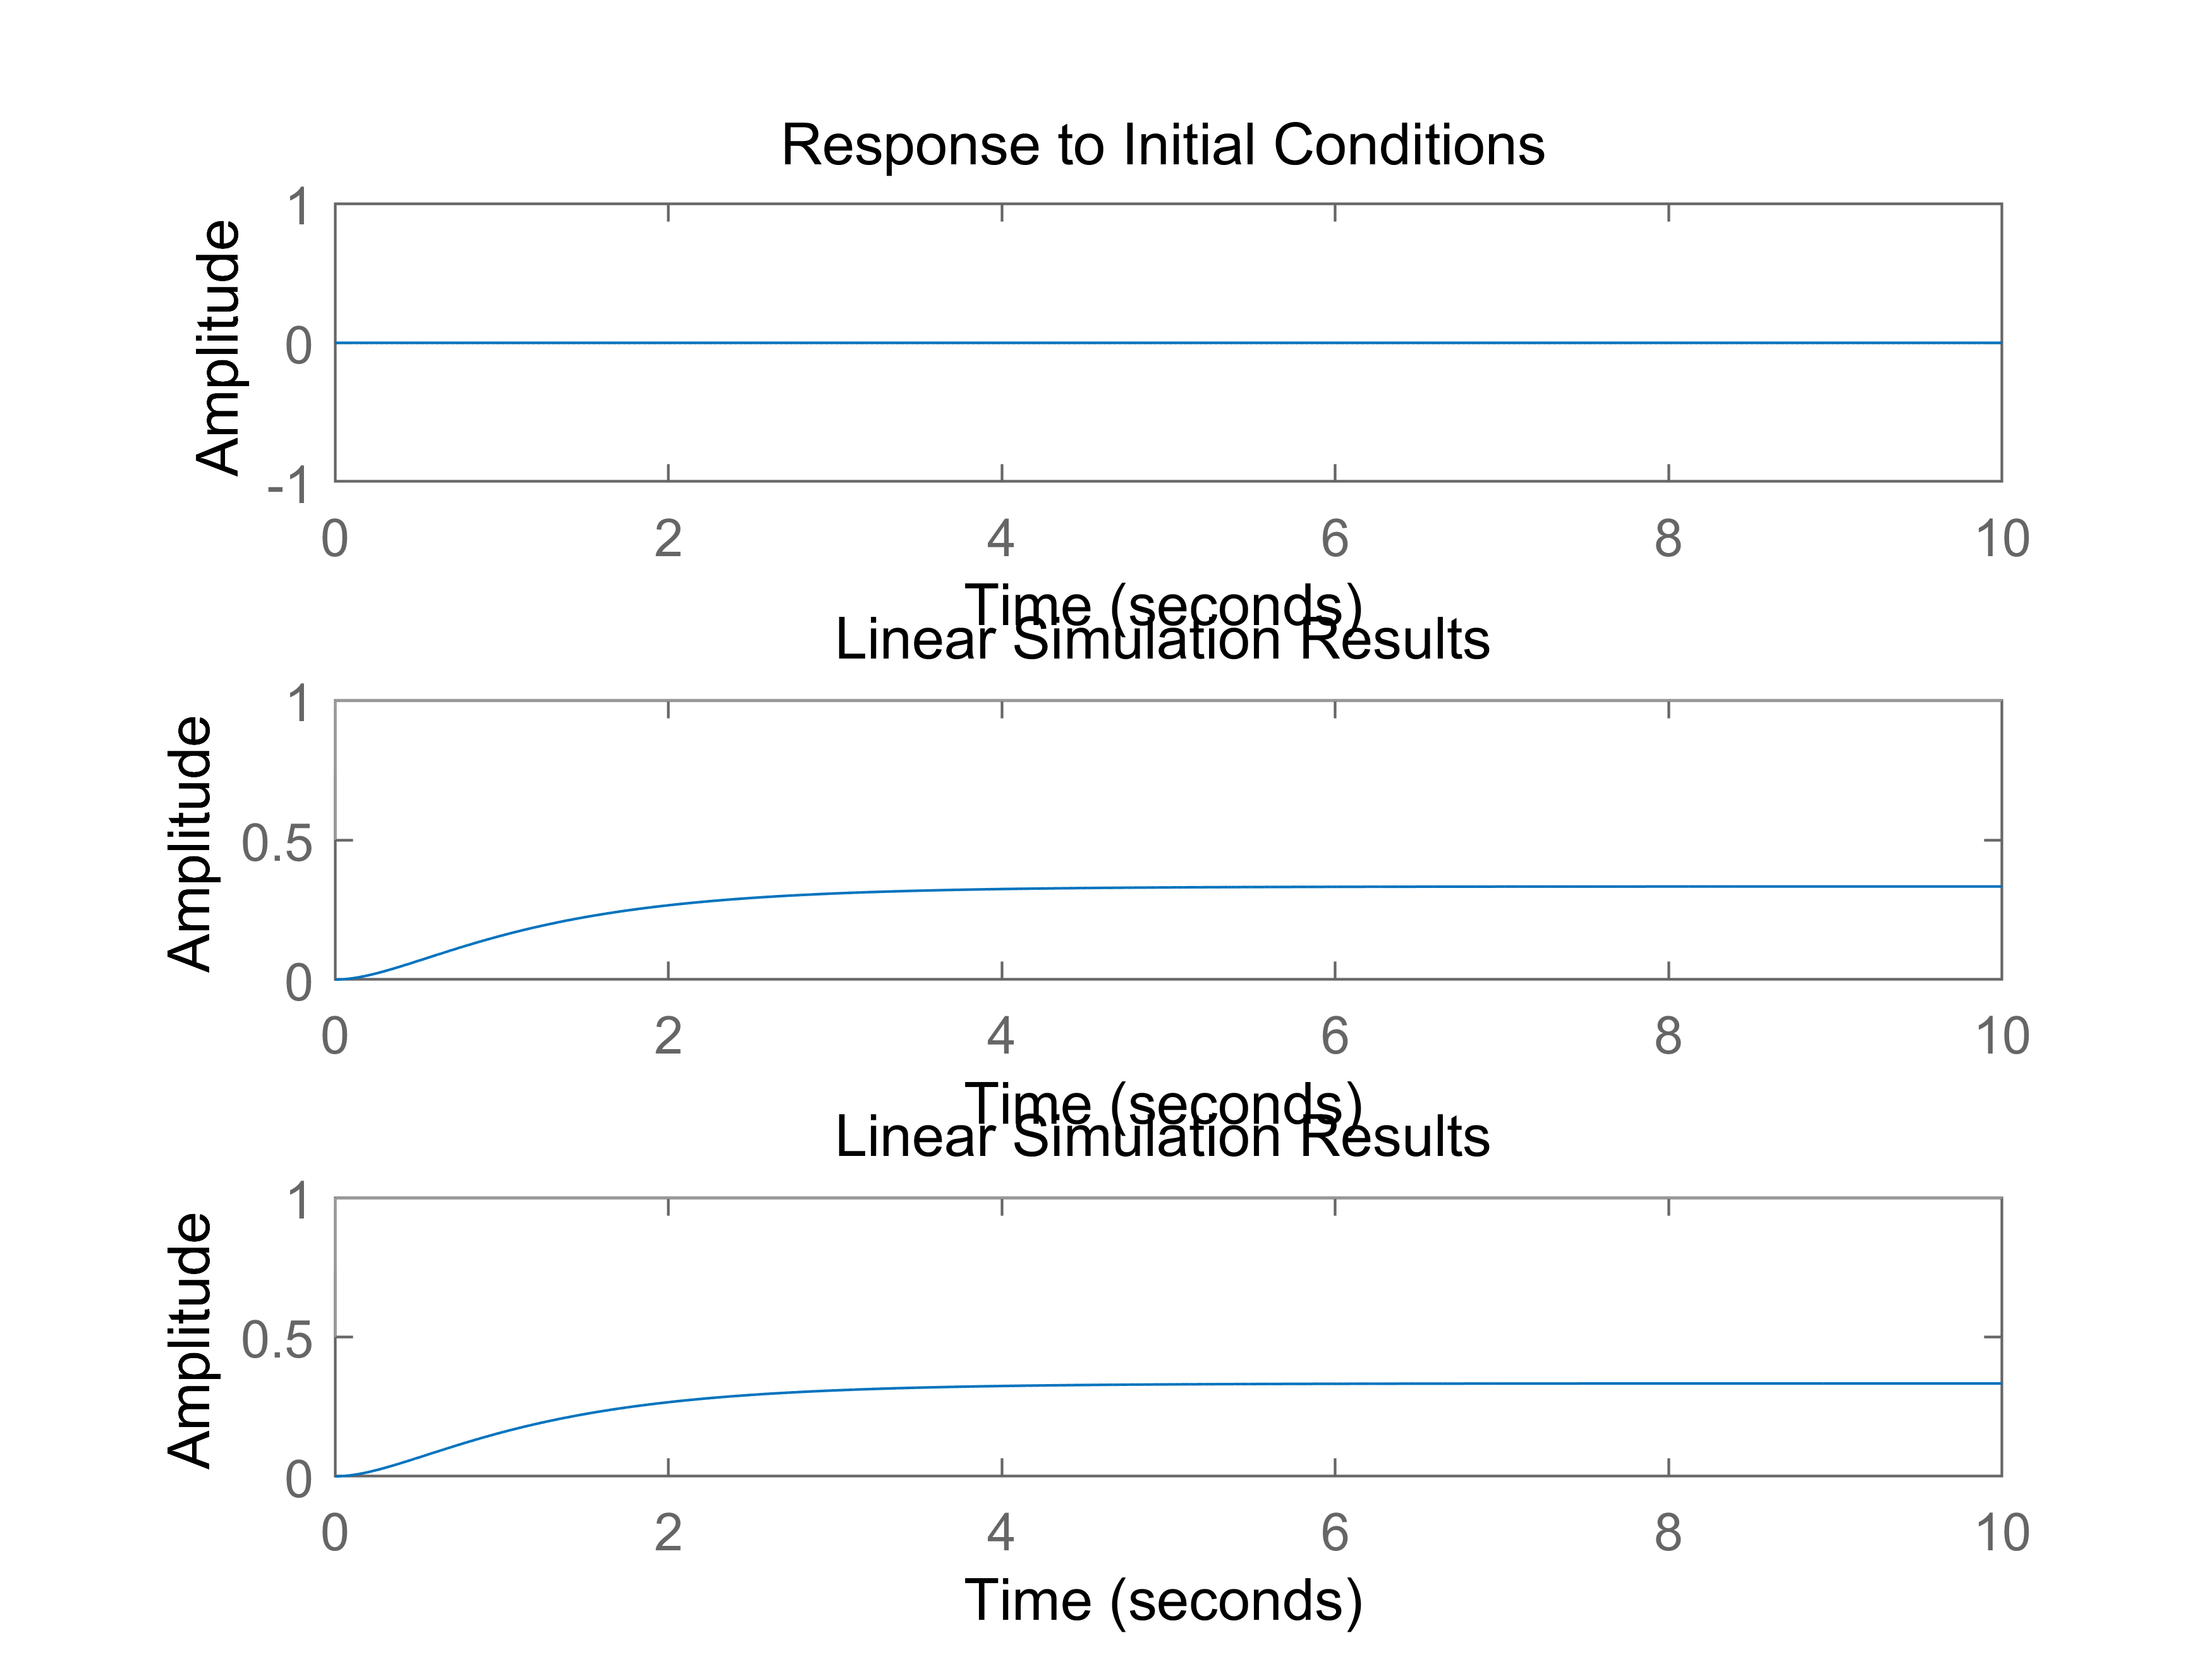
\includegraphics[scale=0.9]{数值1-1.png}
symbolic method\\
\begin{lstlisting}
	clear all;
	eq1='D2y+4*Dy+3*y=heaviside(t)';
	cond='y(-0.01)=0,Dy(-0.01)=0';
	result=dsolve(eq1,cond);
	simplify(result);
	ezplot(result,[0:0.01:10]) ;
	title('y(t)')	
\end{lstlisting}
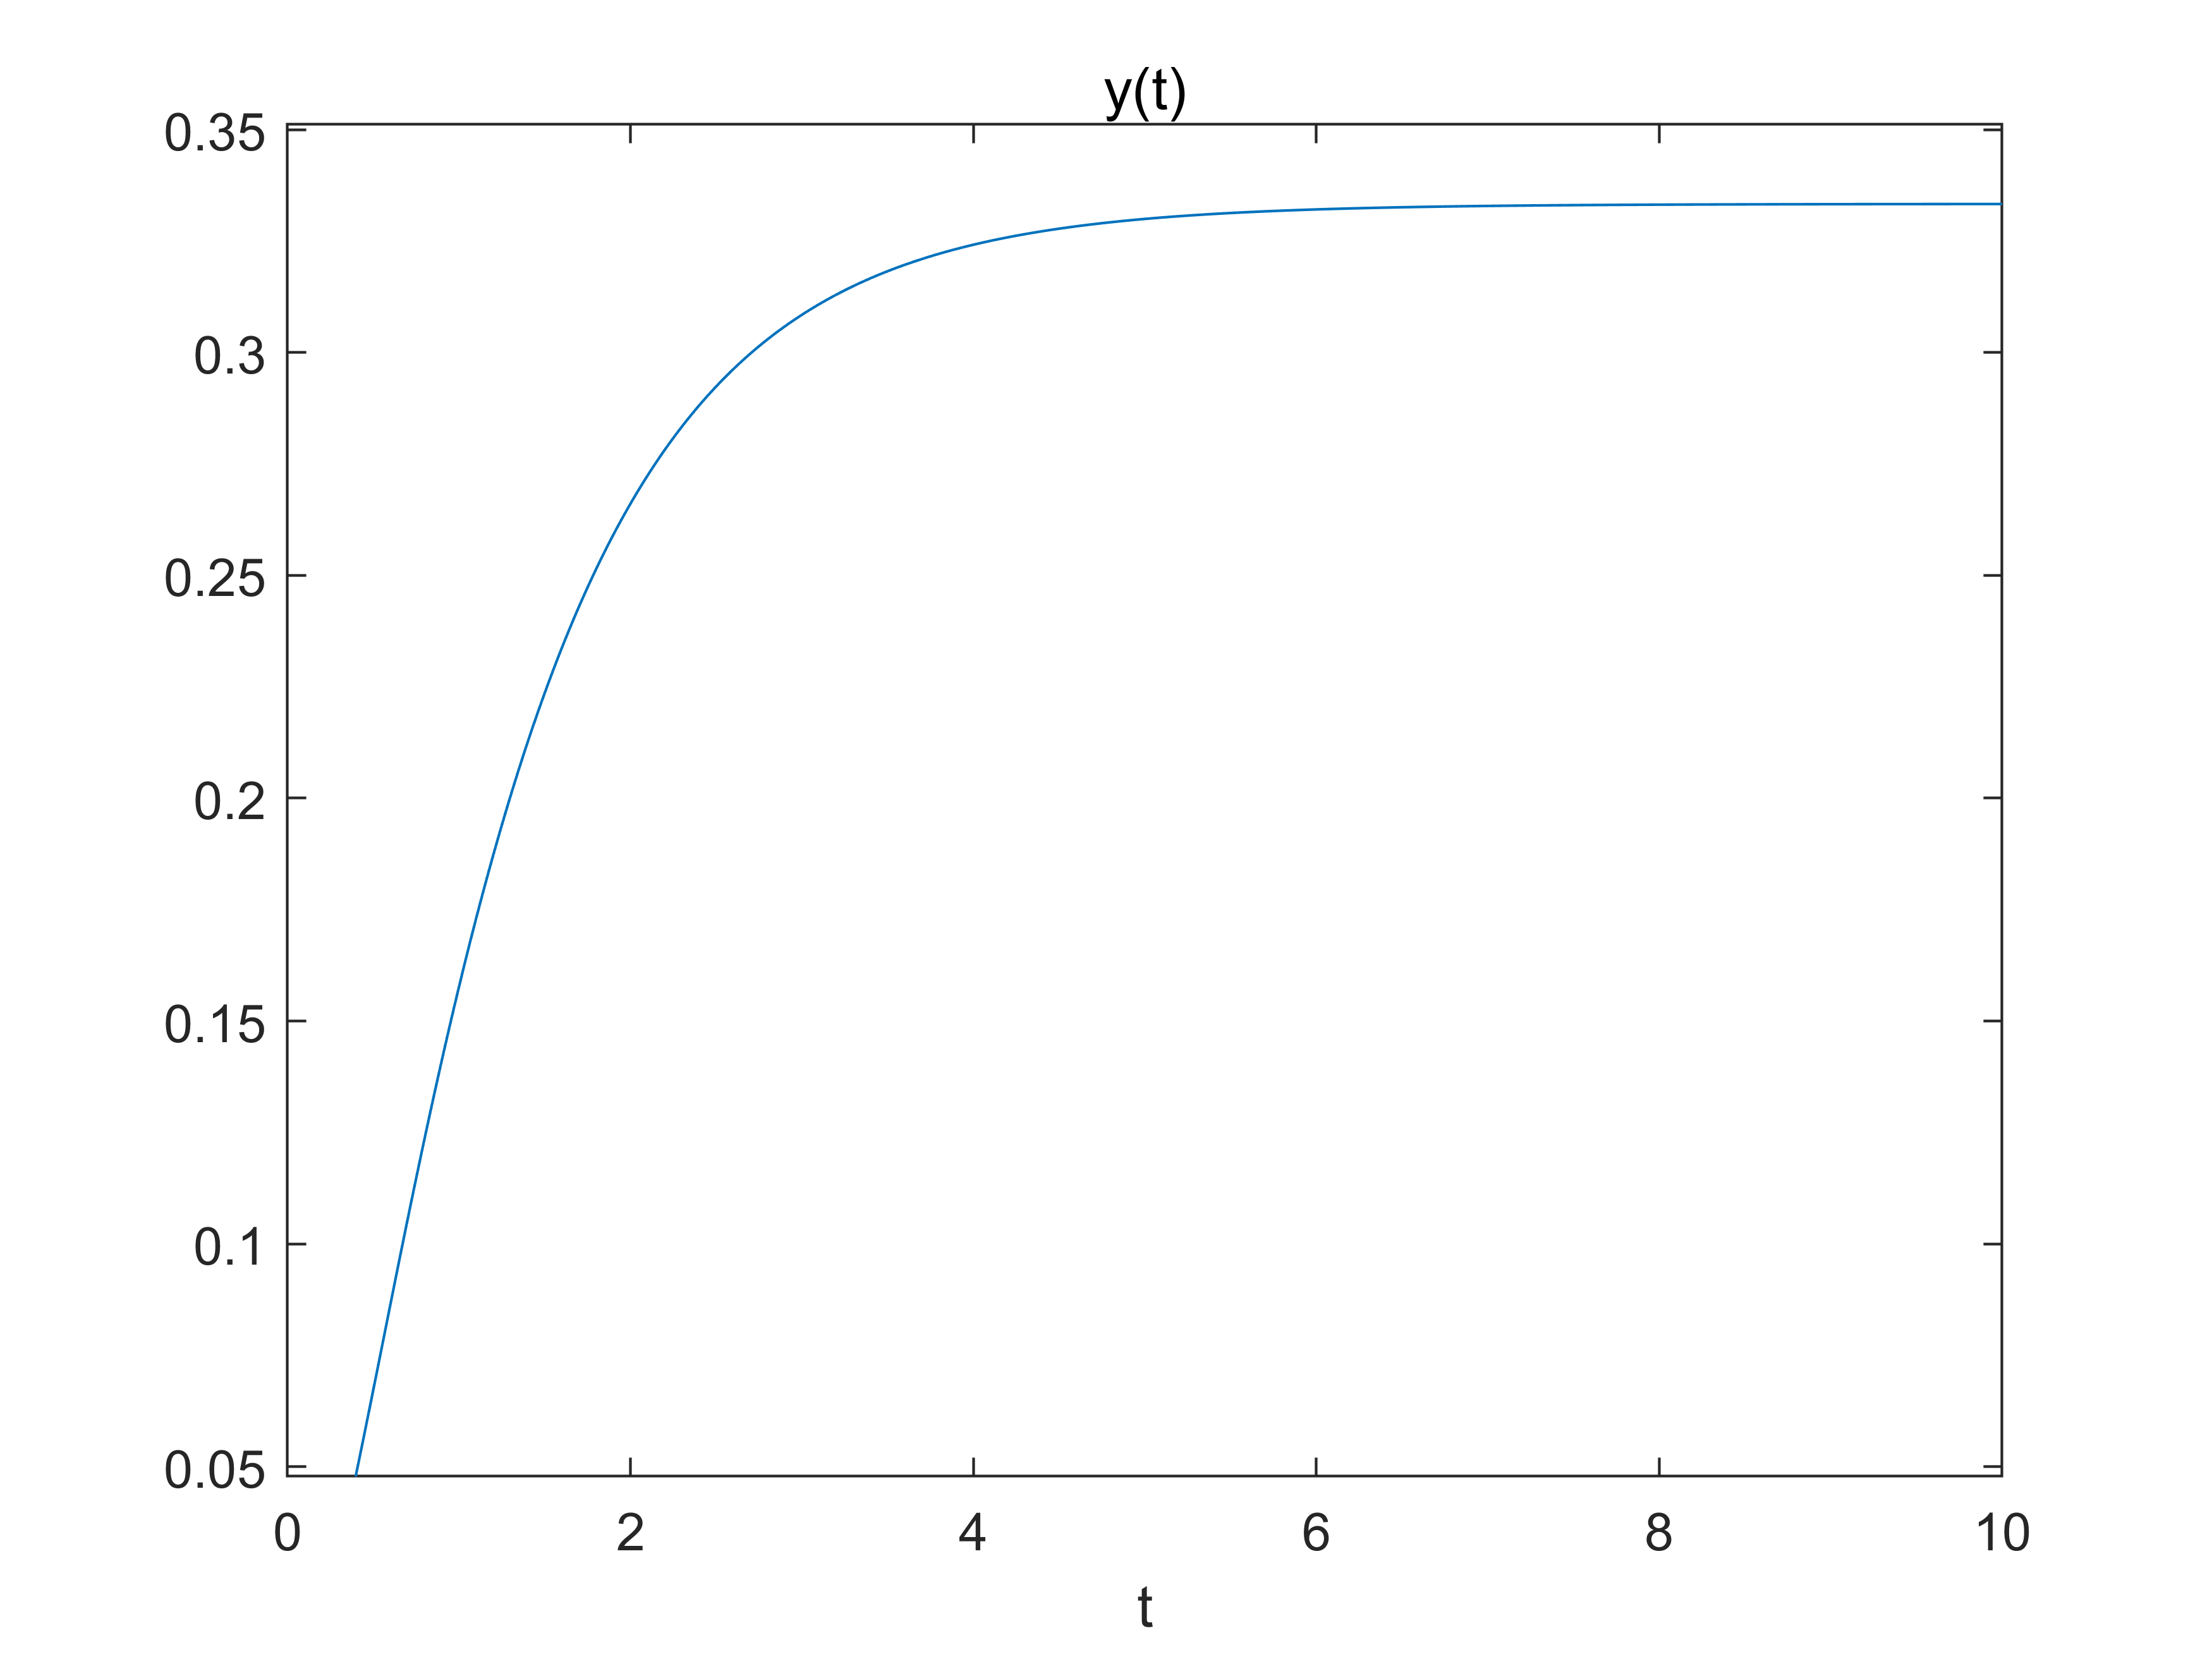
\includegraphics[scale=1]{符号法/1-1.png}\\
Convolution method\\
\begin{lstlisting}
function [f,t]=ctsconv(f1,f2,t1,t2,dt)
f=conv(f1,f2);
f=f*dt;
ts=min(t1)+min(t2);
te=max(t1)+max(t2);
t=ts:dt:te;
plot(t,f);
grid on;
title('f(t)')
end

clear all;
dt = 0.001 ;
t1 = 0:dt:10 ;
f1 = heaviside(t1) ;
t2 = t1 ;
b = [0 0 1] ;
a = [1 4 3] ;
[A B C D] = tf2ss(b,a) ;
sys = ss(A,B,C,D) ;
f2 = impulse(sys,t2) ;
[f,t] = ctsconv(f1,f2,t1,t2,dt) ;
subplot(3,1,1)
plot(t1,f1) ;
hold on;
axis([0,10,0,2])
grid on ;
title('u(t)') ;
subplot(3,1,2)
plot(t2,f2) ;
grid on ;
title('h(t)') ;
subplot(3,1,3)
plot(t,f) ;
hold on;
axis([0,10,0,0.5])
grid on ;
title('f(t)*h(t)') ;

1-2
clear all;
dt = 0.001 ;
t1 = 0:dt:10 ;
f1 = exp(-t1).*heaviside(t1);
t2 = t1 ;
b = [0 0 1] ;
a = [1 4 3] ;
[A B C D] = tf2ss(b,a) ;
sys = ss(A,B,C,D) ;
f2 = impulse(sys,t2) ;
[f,t] = ctsconv(f1,f2,t1,t2,dt) ;
subplot(3,1,1)
plot(t1,f1) ;
hold on;
axis([0,10,0,2])
grid on ;
title('$f(t)=u(t)e^{-t}$','Interpreter','Latex') ;
subplot(3,1,2)
plot(t2,f2) ;
grid on ;
title('h(t)') ;
subplot(3,1,3)
plot(t,f) ;
hold on;
axis([0,10,0,0.5])
grid on ;
title('f(t)*h(t)') ;
\end{lstlisting}
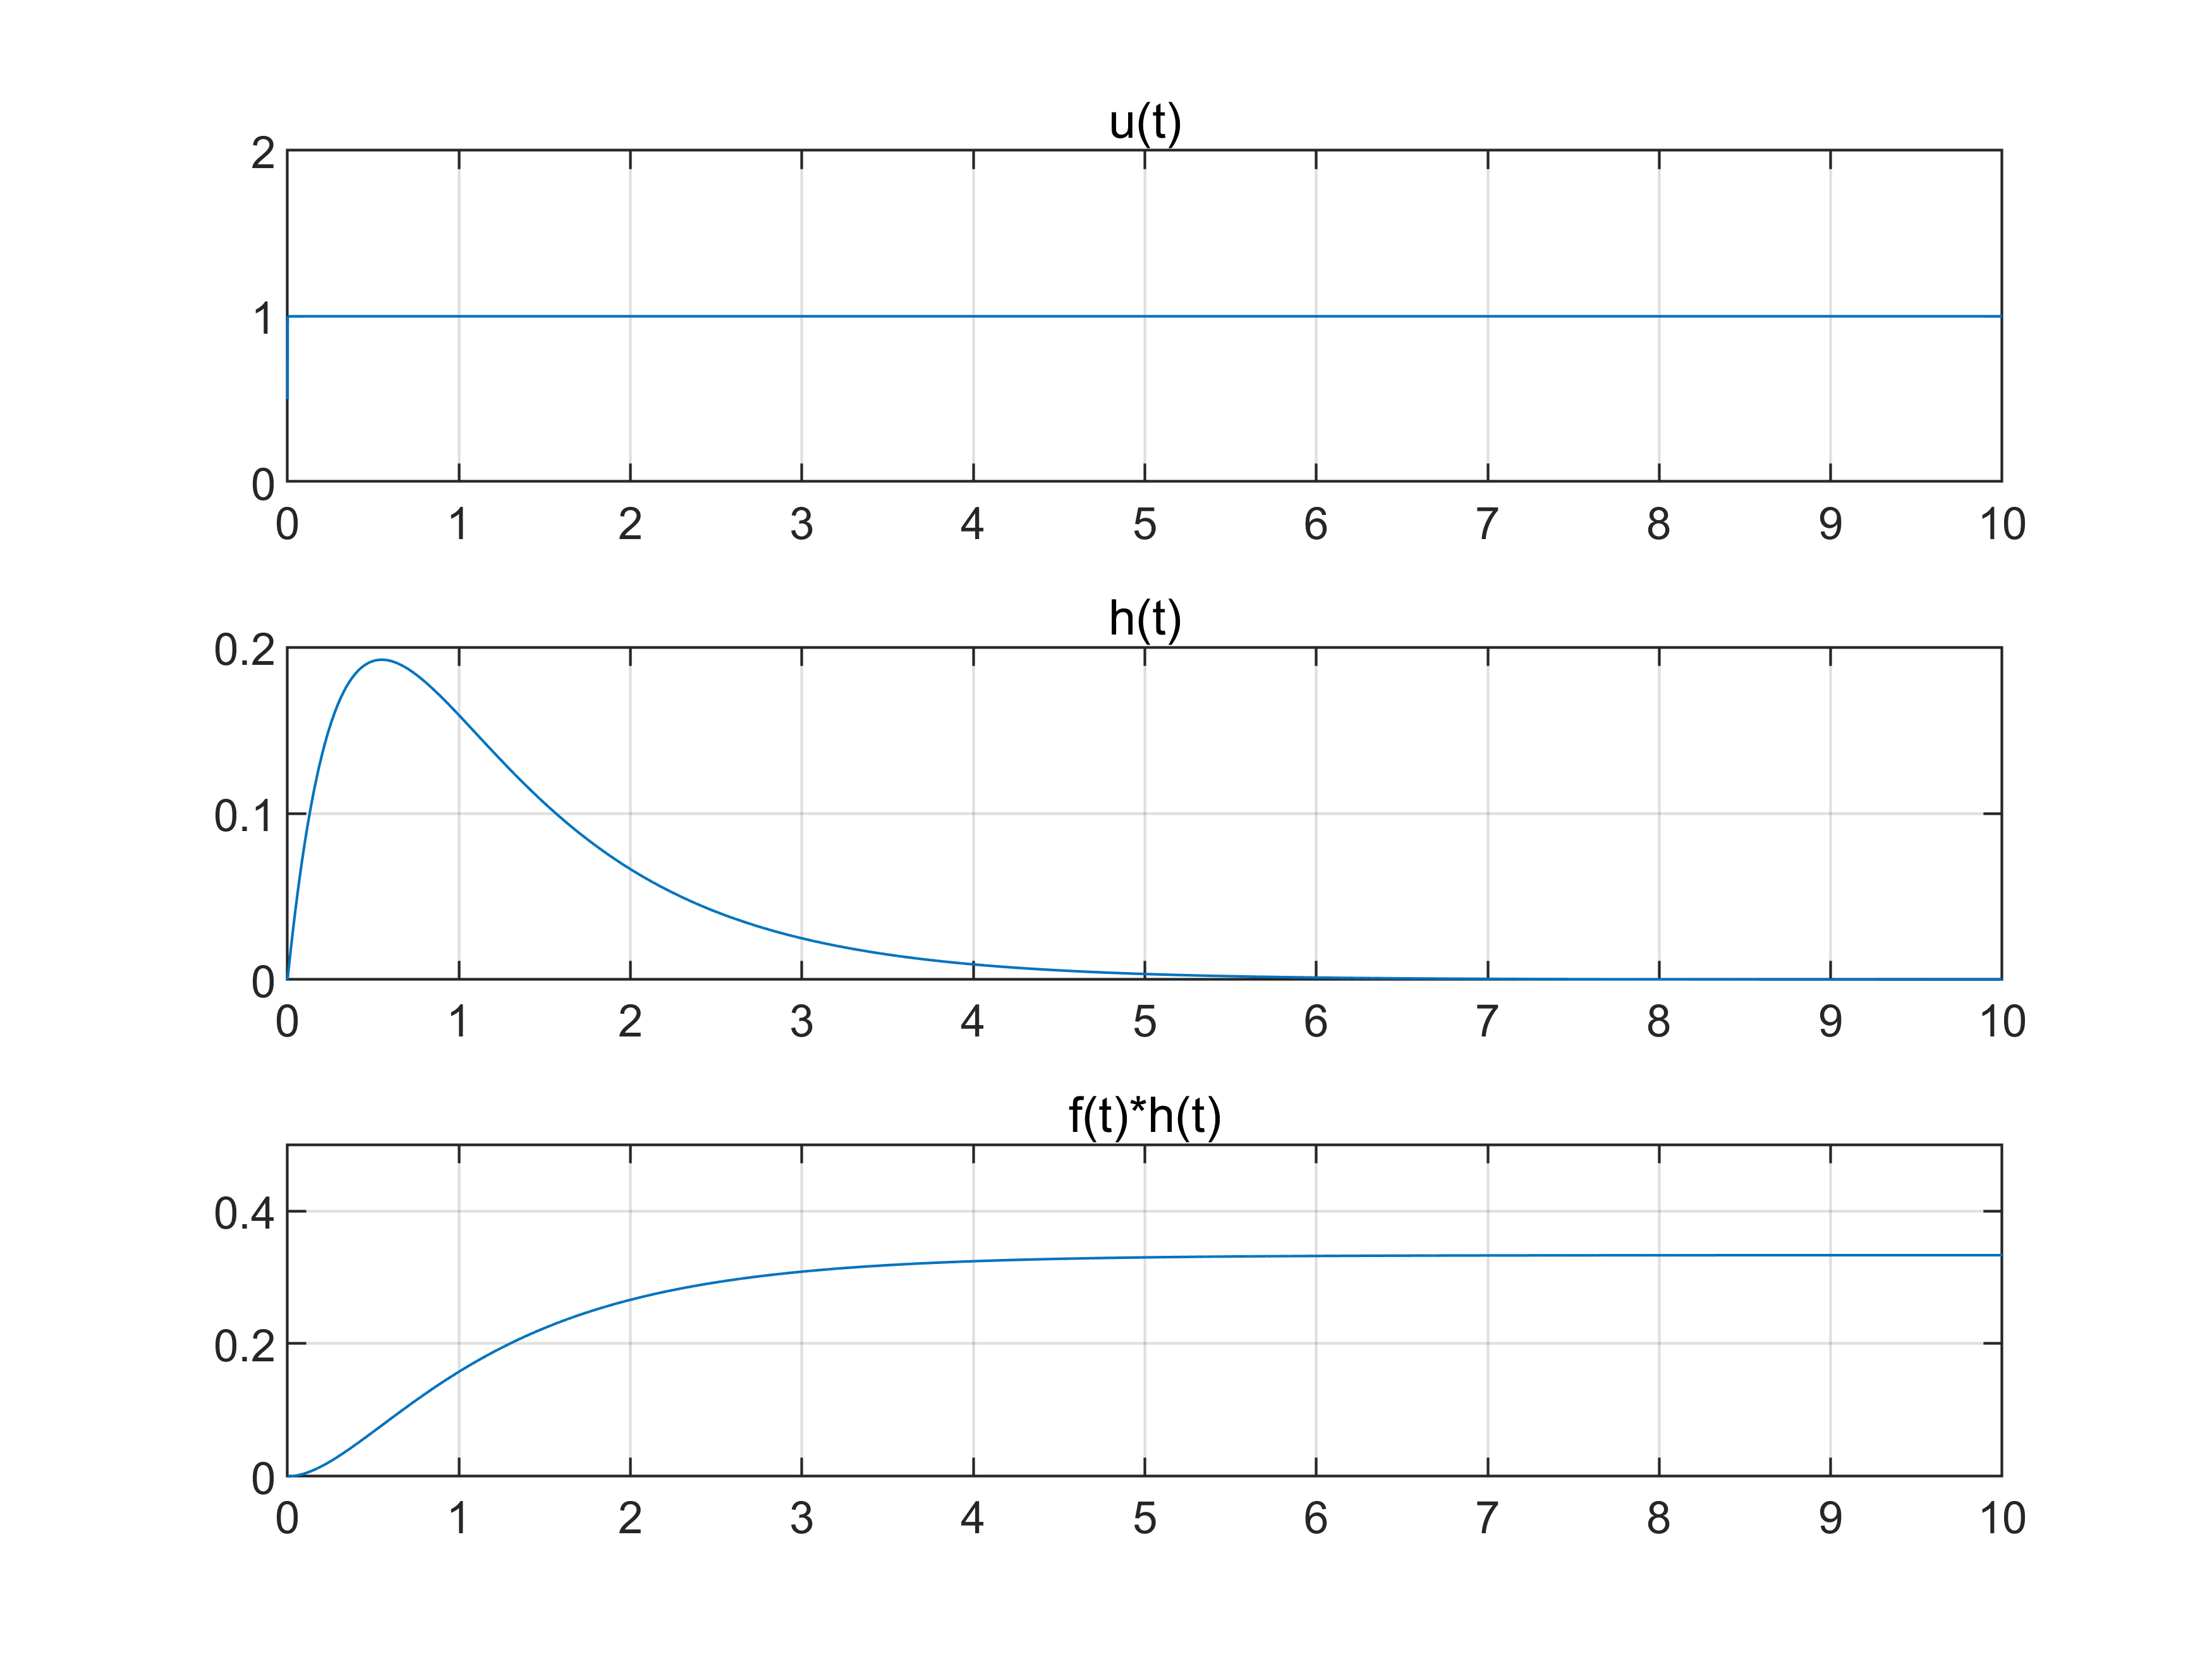
\includegraphics[scale=1]{1卷积.png}\\\\
(1-2)\\
Numberical method:\\
\begin{lstlisting}
	clear all;
	a=[1 4 4];
	b=[0 1 3];
	t=0:0.001:10;
	x=heaviside(t),*exp(-t);
	rc=[0,0];
	sys=tf(b,a)
	[A,B,C,D]=tf2ss(b,a)
	subplot(3,1,1),initial(A,B,C,D,rc,t) %零输入响应
	subplot(3,1,2),lsim(b,a,x,t)         %零状态响应
	subplot(3,1,3),lsim(A,B,C,D,x,t,rc)  %全响应,只能用状态系数来表示系统
\end{lstlisting}
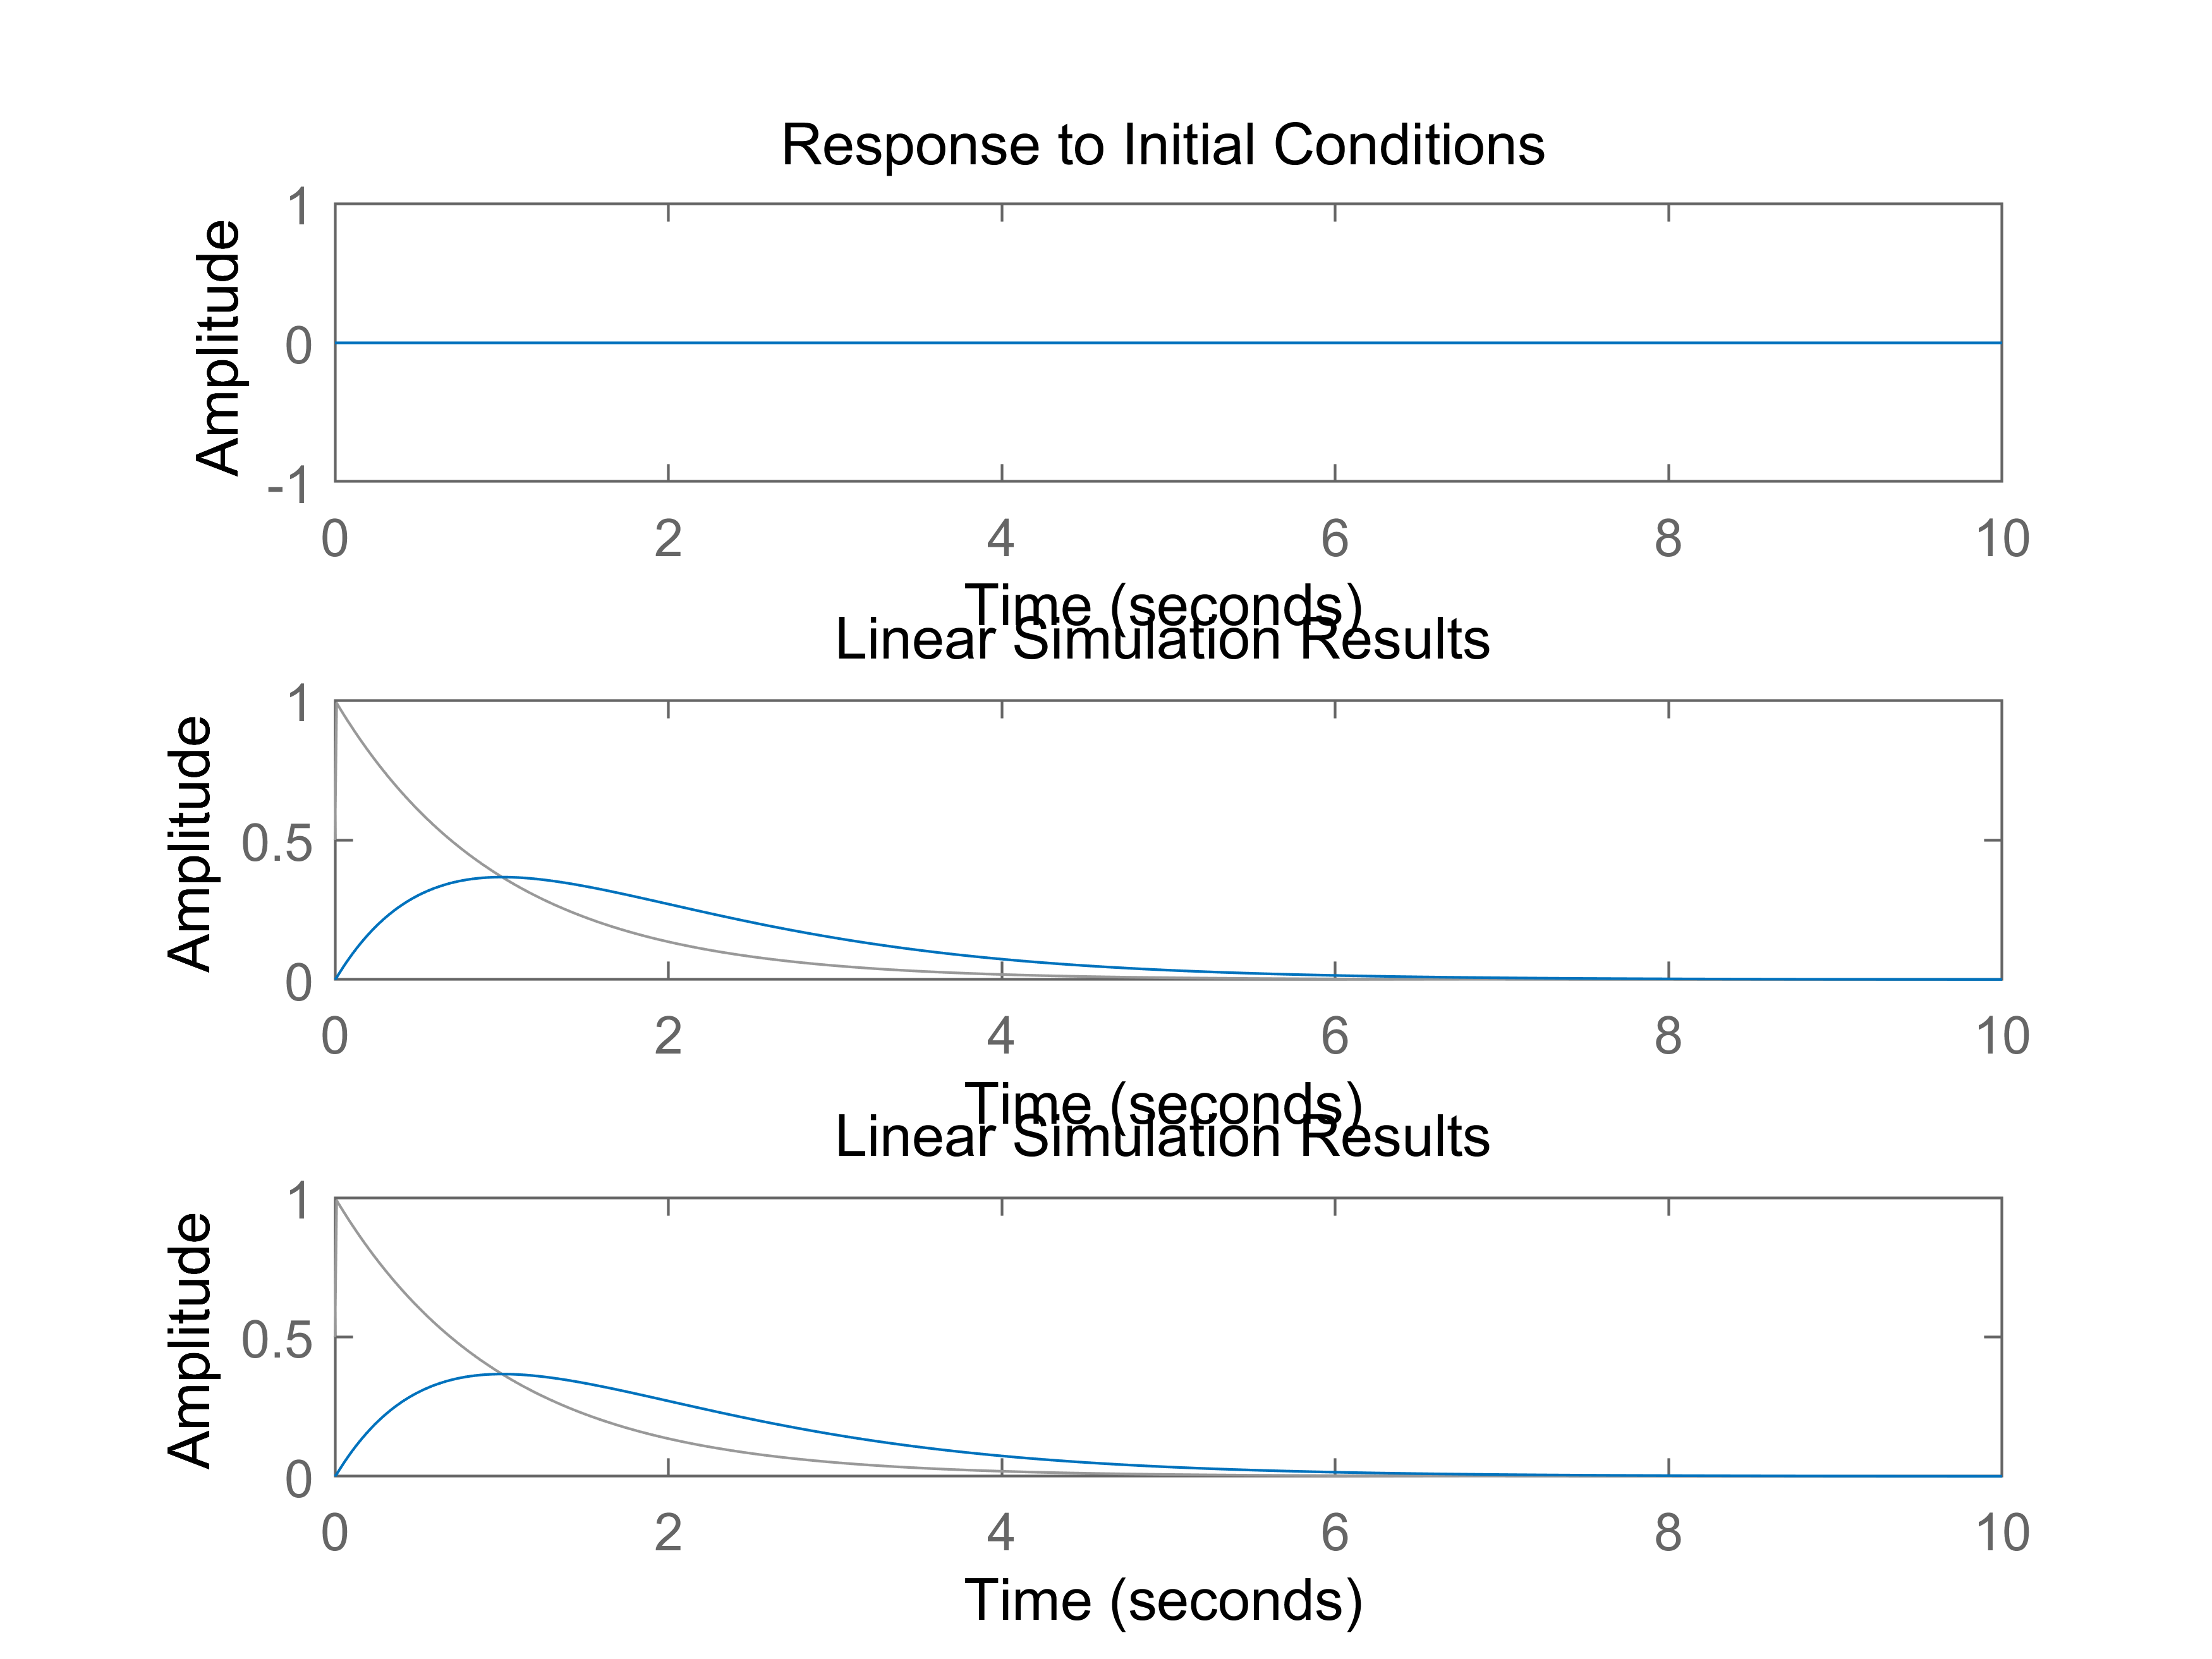
\includegraphics[scale=1]{数值1-2.png}\\
Symbolic method:\\
\begin{lstlisting}
clear all 
eq1 ='D2y+4*Dy+4*y=Dx+3*x' ;
eq2 = 'x=heaviside(t)*exp(-t)' ;
cond = 'y(-0.01)=0,Dy(-0.01)=0,D2y(-0.01)=0';
ans1 = dsolve( eq1,eq2,cond); 
simplify(ans1.y);
ezplot(ans1.y,[0:0.01:10]) ;
title('y(t)');
\end{lstlisting}
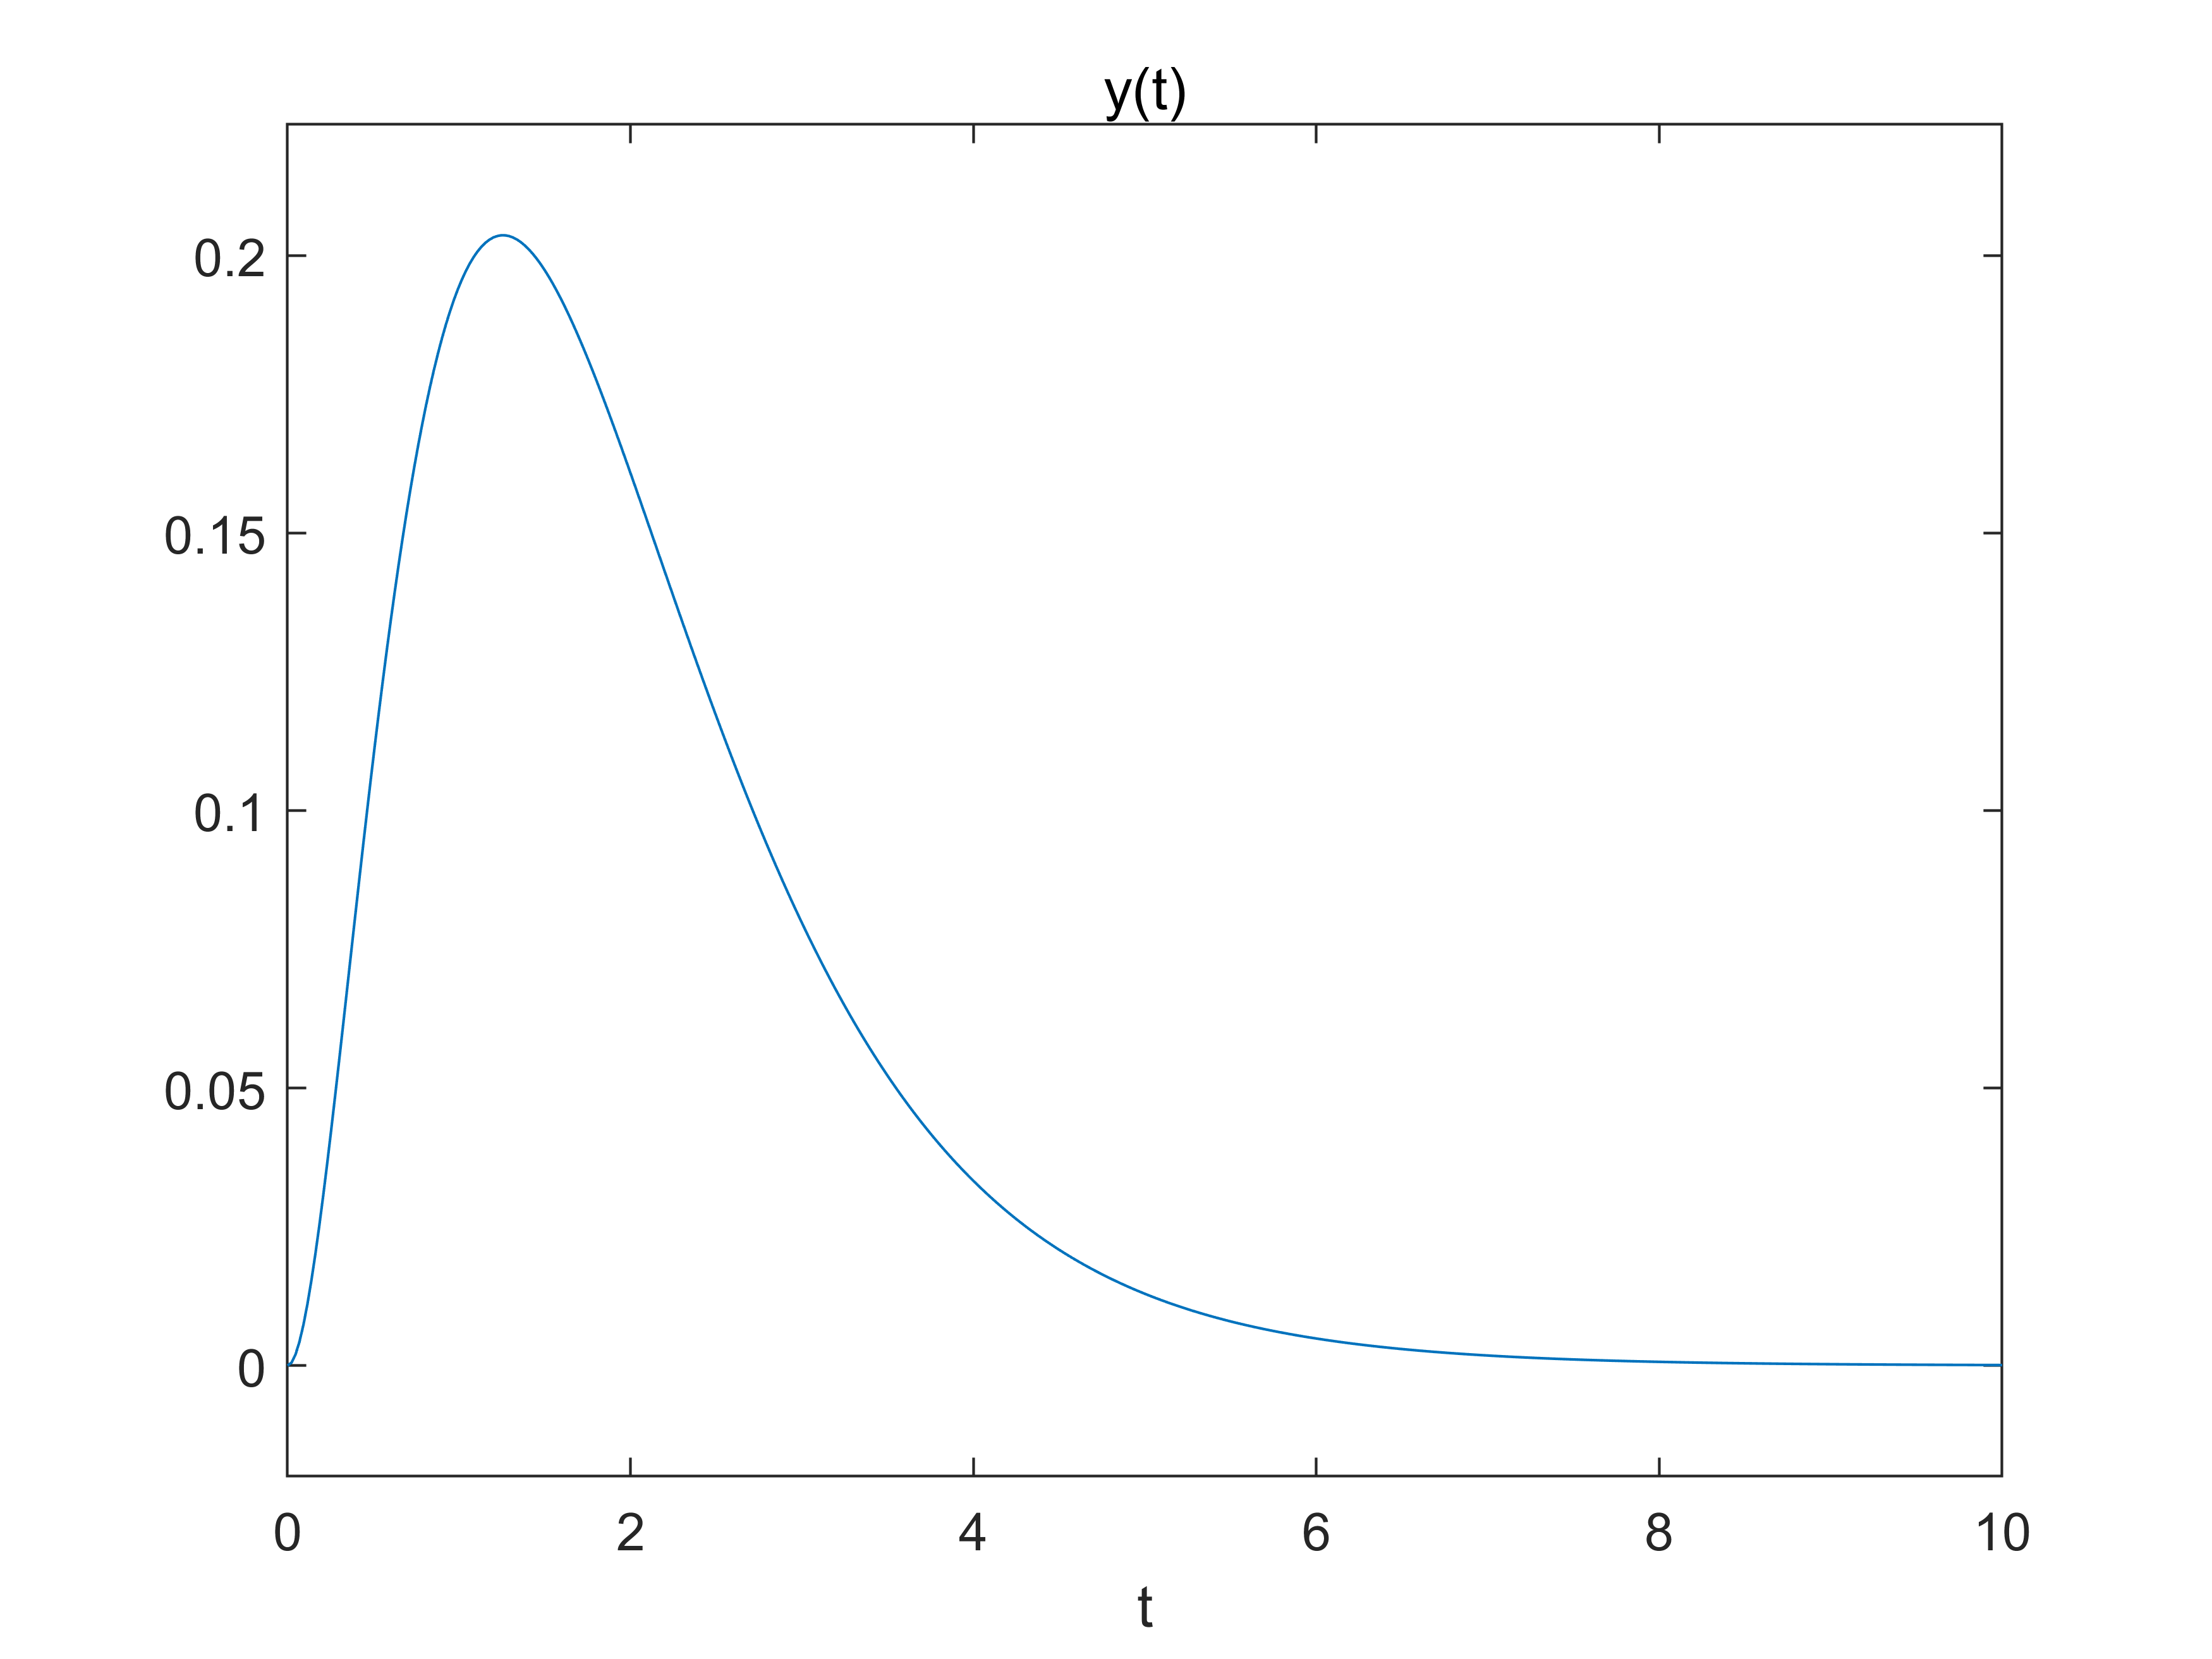
\includegraphics[scale=1]{符号法/1-2.png}\\
Convolution method:\\
\begin{lstlisting}
	clear all;
	dt = 0.001 ;
	t1 = 0:dt:10 ;
	f1 = exp(-t1).*heaviside(t1);
	t2 = t1 ;
	b = [0 0 1] ;
	a = [1 4 3] ;
	[A B C D] = tf2ss(b,a) ;
	sys = ss(A,B,C,D) ;
	f2 = impulse(sys,t2) ;
	[f,t] = ctsconv(f1,f2,t1,t2,dt) ;
	subplot(3,1,1)
	plot(t1,f1) ;
	hold on;
	axis([0,10,0,2])
	grid on ;
	title('$f(t)=u(t)e^{-t}$','Interpreter','Latex') ;
	subplot(3,1,2)
	plot(t2,f2) ;
	grid on ;
	title('h(t)') ;
	subplot(3,1,3)
	plot(t,f) ;
	hold on;
	axis([0,10,0,0.5])
	grid on ;
	title('f(t)*h(t)') ;
\end{lstlisting}	
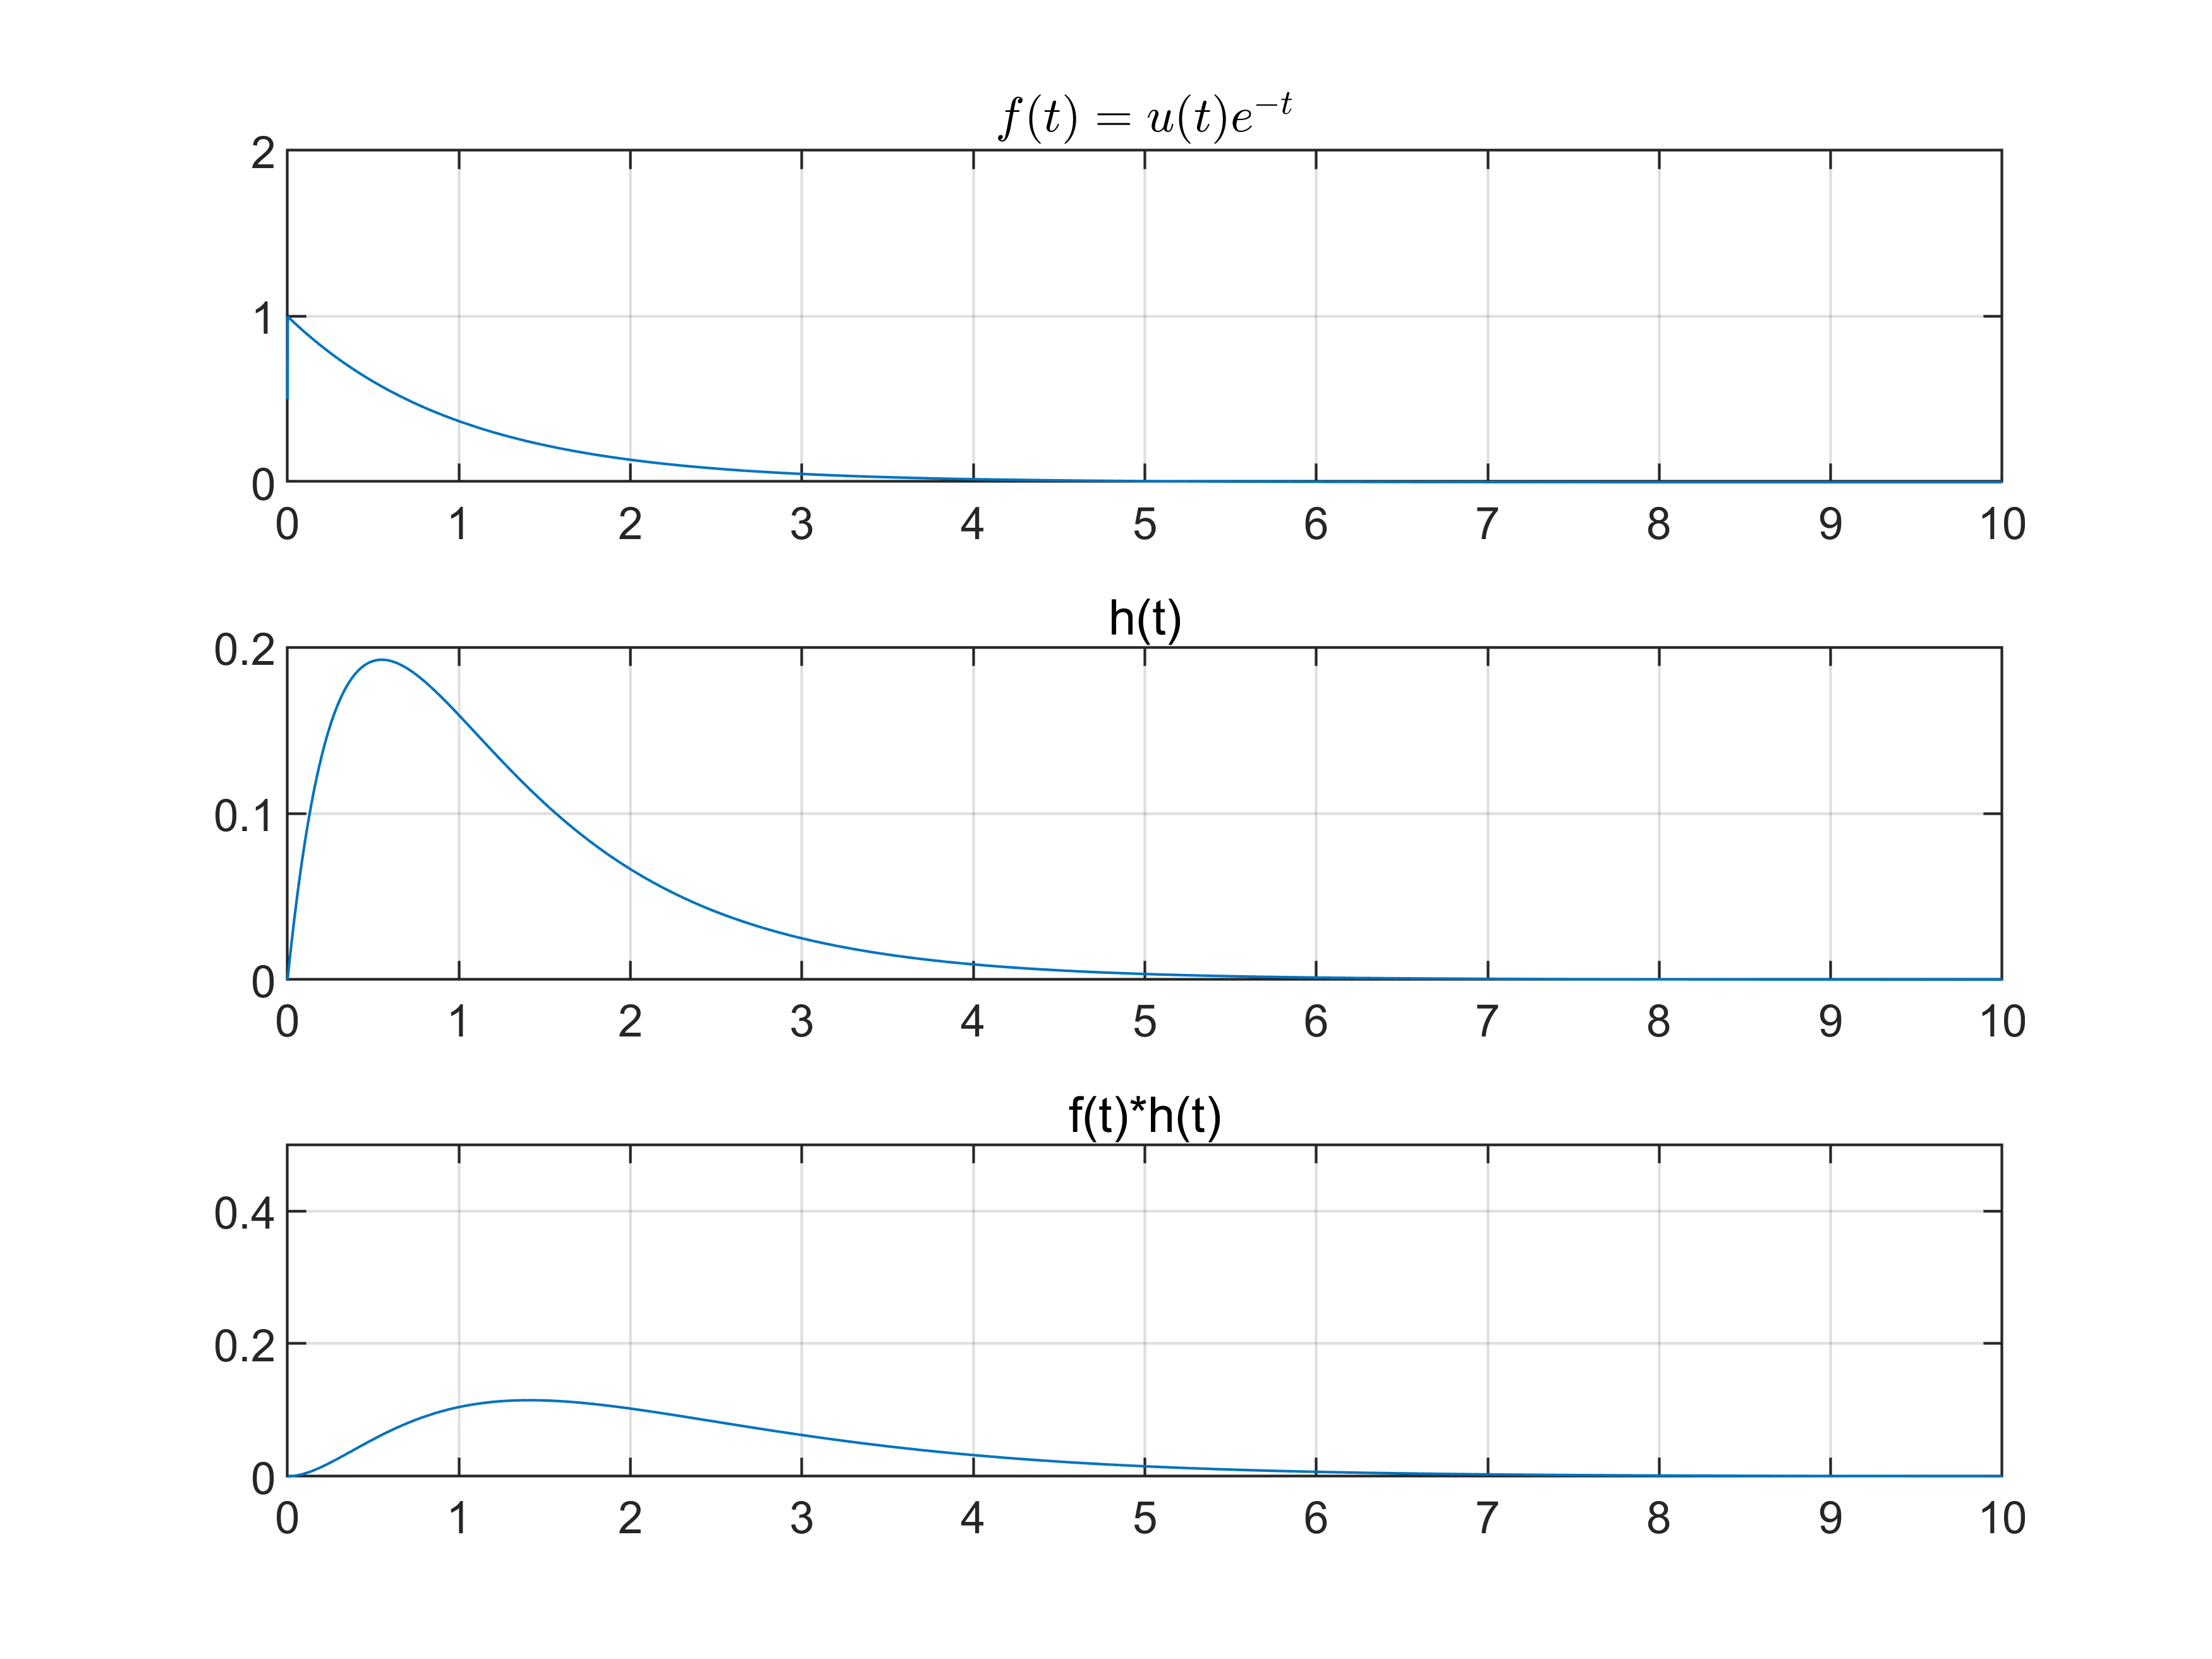
\includegraphics[scale=1]{1-2卷积.png}
\section{Problem 2}
\subsection{Description}
Differential equations and excitation signals for known systems, zero-state response (with symbolism, numerical method, convolution integral method)
$$
\begin{aligned}
y''(t)+4y'(t)+3y(t)=f'(t)+f(t),f(t)=e^{-2t}u(t)\\
y(0)=2,y'(0)=1
\end{aligned}
$$
Numberical method:\\
\begin{lstlisting}
	clear all;
	a=[1 4 3];
	b=[0 1 1];
	t=0:0.001:10;
	x=heaviside(t),*exp(-2*t);
	rc=[2,1];
	sys=tf(b,a)
	[A,B,C,D]=tf2ss(b,a)
	subplot(3,1,1),initial(A,B,C,D,rc,t) %零输入响应
	subplot(3,1,2),lsim(b,a,x,t)         %零状态响应
	subplot(3,1,3),lsim(A,B,C,D,x,t,rc)  %全响应,只能用状态系数来表示系统	
\end{lstlisting}
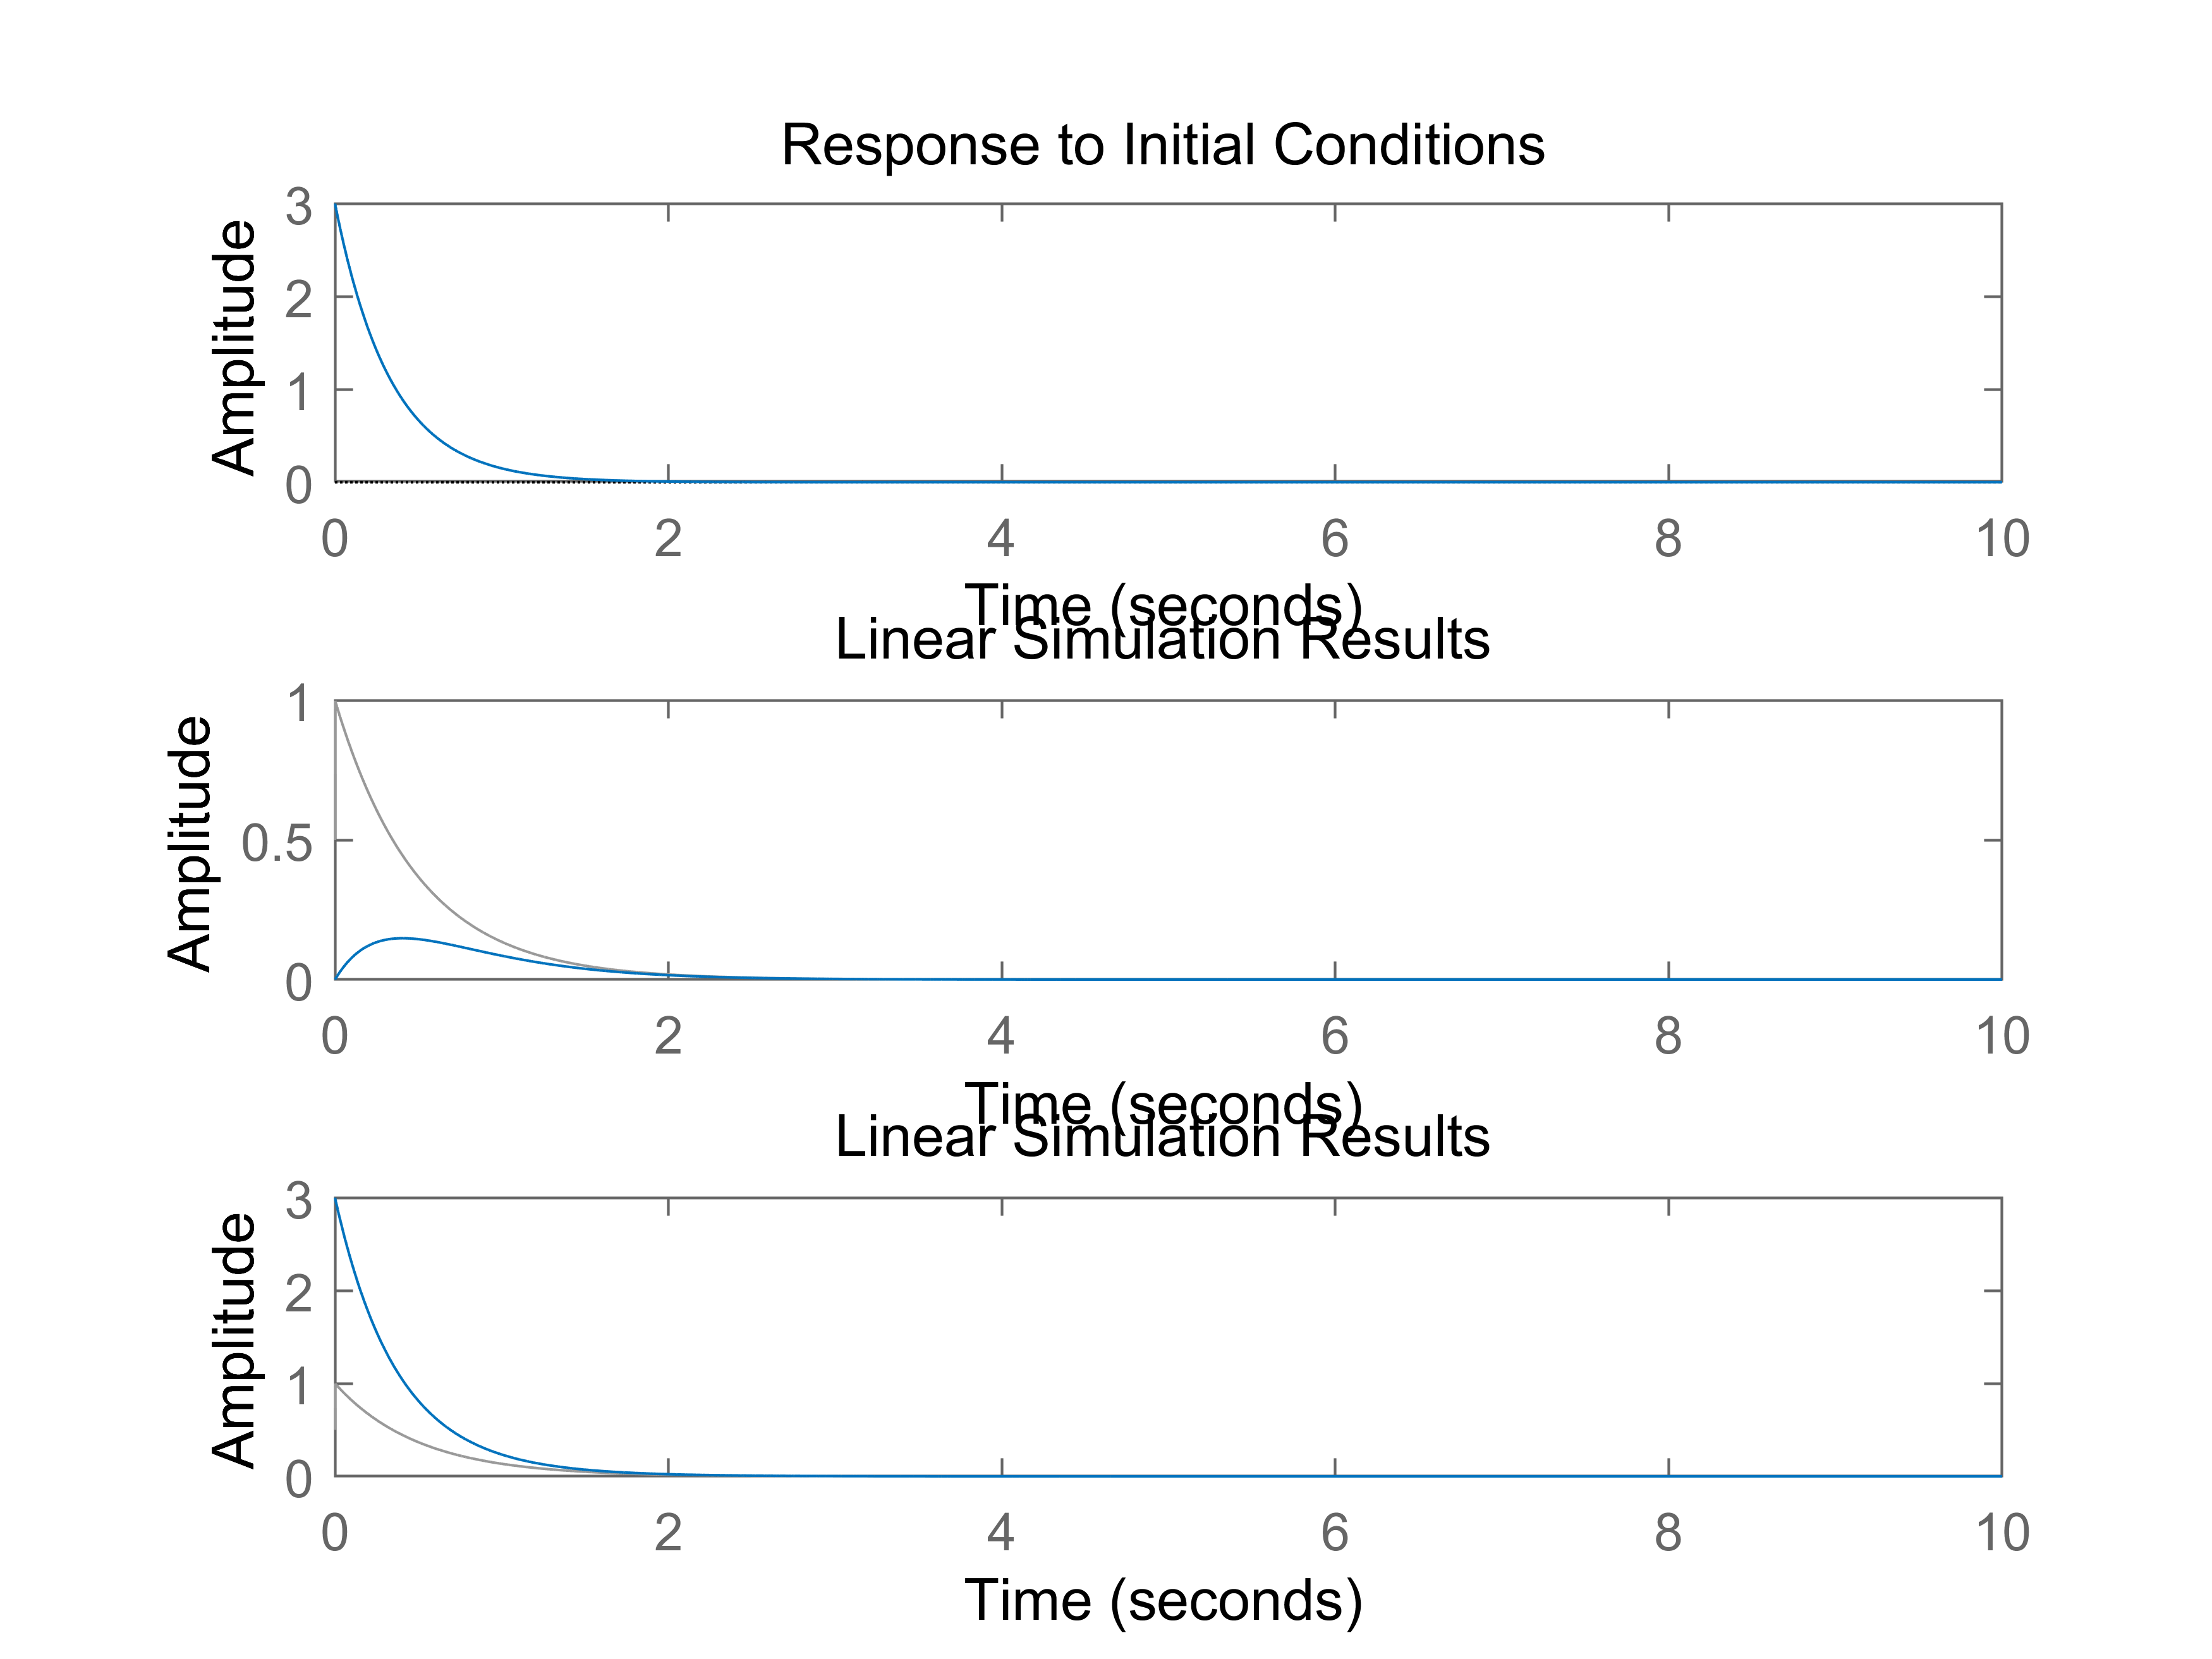
\includegraphics[scale=1]{数值2.png}\\
Symbolic method:\\
\begin{lstlisting}
	% 2
	clear all 
	% 零状态
	eq1 ='D2y+4*Dy+3*y=Dx+x' ;
	eq2 = 'x=heaviside(t)*exp(-2*t)' ;
	cond = 'y(-0.01)=0,Dy(-0.01)=0,D2y(-0.01)=0';
	ans1 = dsolve( eq1,eq2,cond); 
	simplify(ans1.y);
	ezplot(ans1.y,[0:0.01:10]) ;
	title('$y_{zs}(t)$','Interpreter','Latex');
	
	2
	clear all;
	%零输入响应
	eq1_1 ='D2y+4*Dy+3=0' ;
	cond_1 ='y(0)=2,Dy(0)=1';
	yzi = dsolve(eq1_1,cond_1);
	ezplot(yzi,[0:0.01:10])
	title('$y_{zi}(t)$','Interpreter','Latex');
	hold on;
	grid on;
	axis([0,10])
	
	
	2
	clear all;
	全响应响应
	eq1_1 ='D2y+4*Dy+3=Dx+x';
	eq2 = 'x=heaviside(t)*exp(-2*t)';
	cond_1 ='y(-0.01)=2,Dy(-0.01)=1';
	y = dsolve(eq1_1,eq2,cond_1);
	ezplot(y.y,[0:0.01:10])
	hold on;
	grid on;
	title('$y(t)$','Interpreter','Latex');
\end{lstlisting}
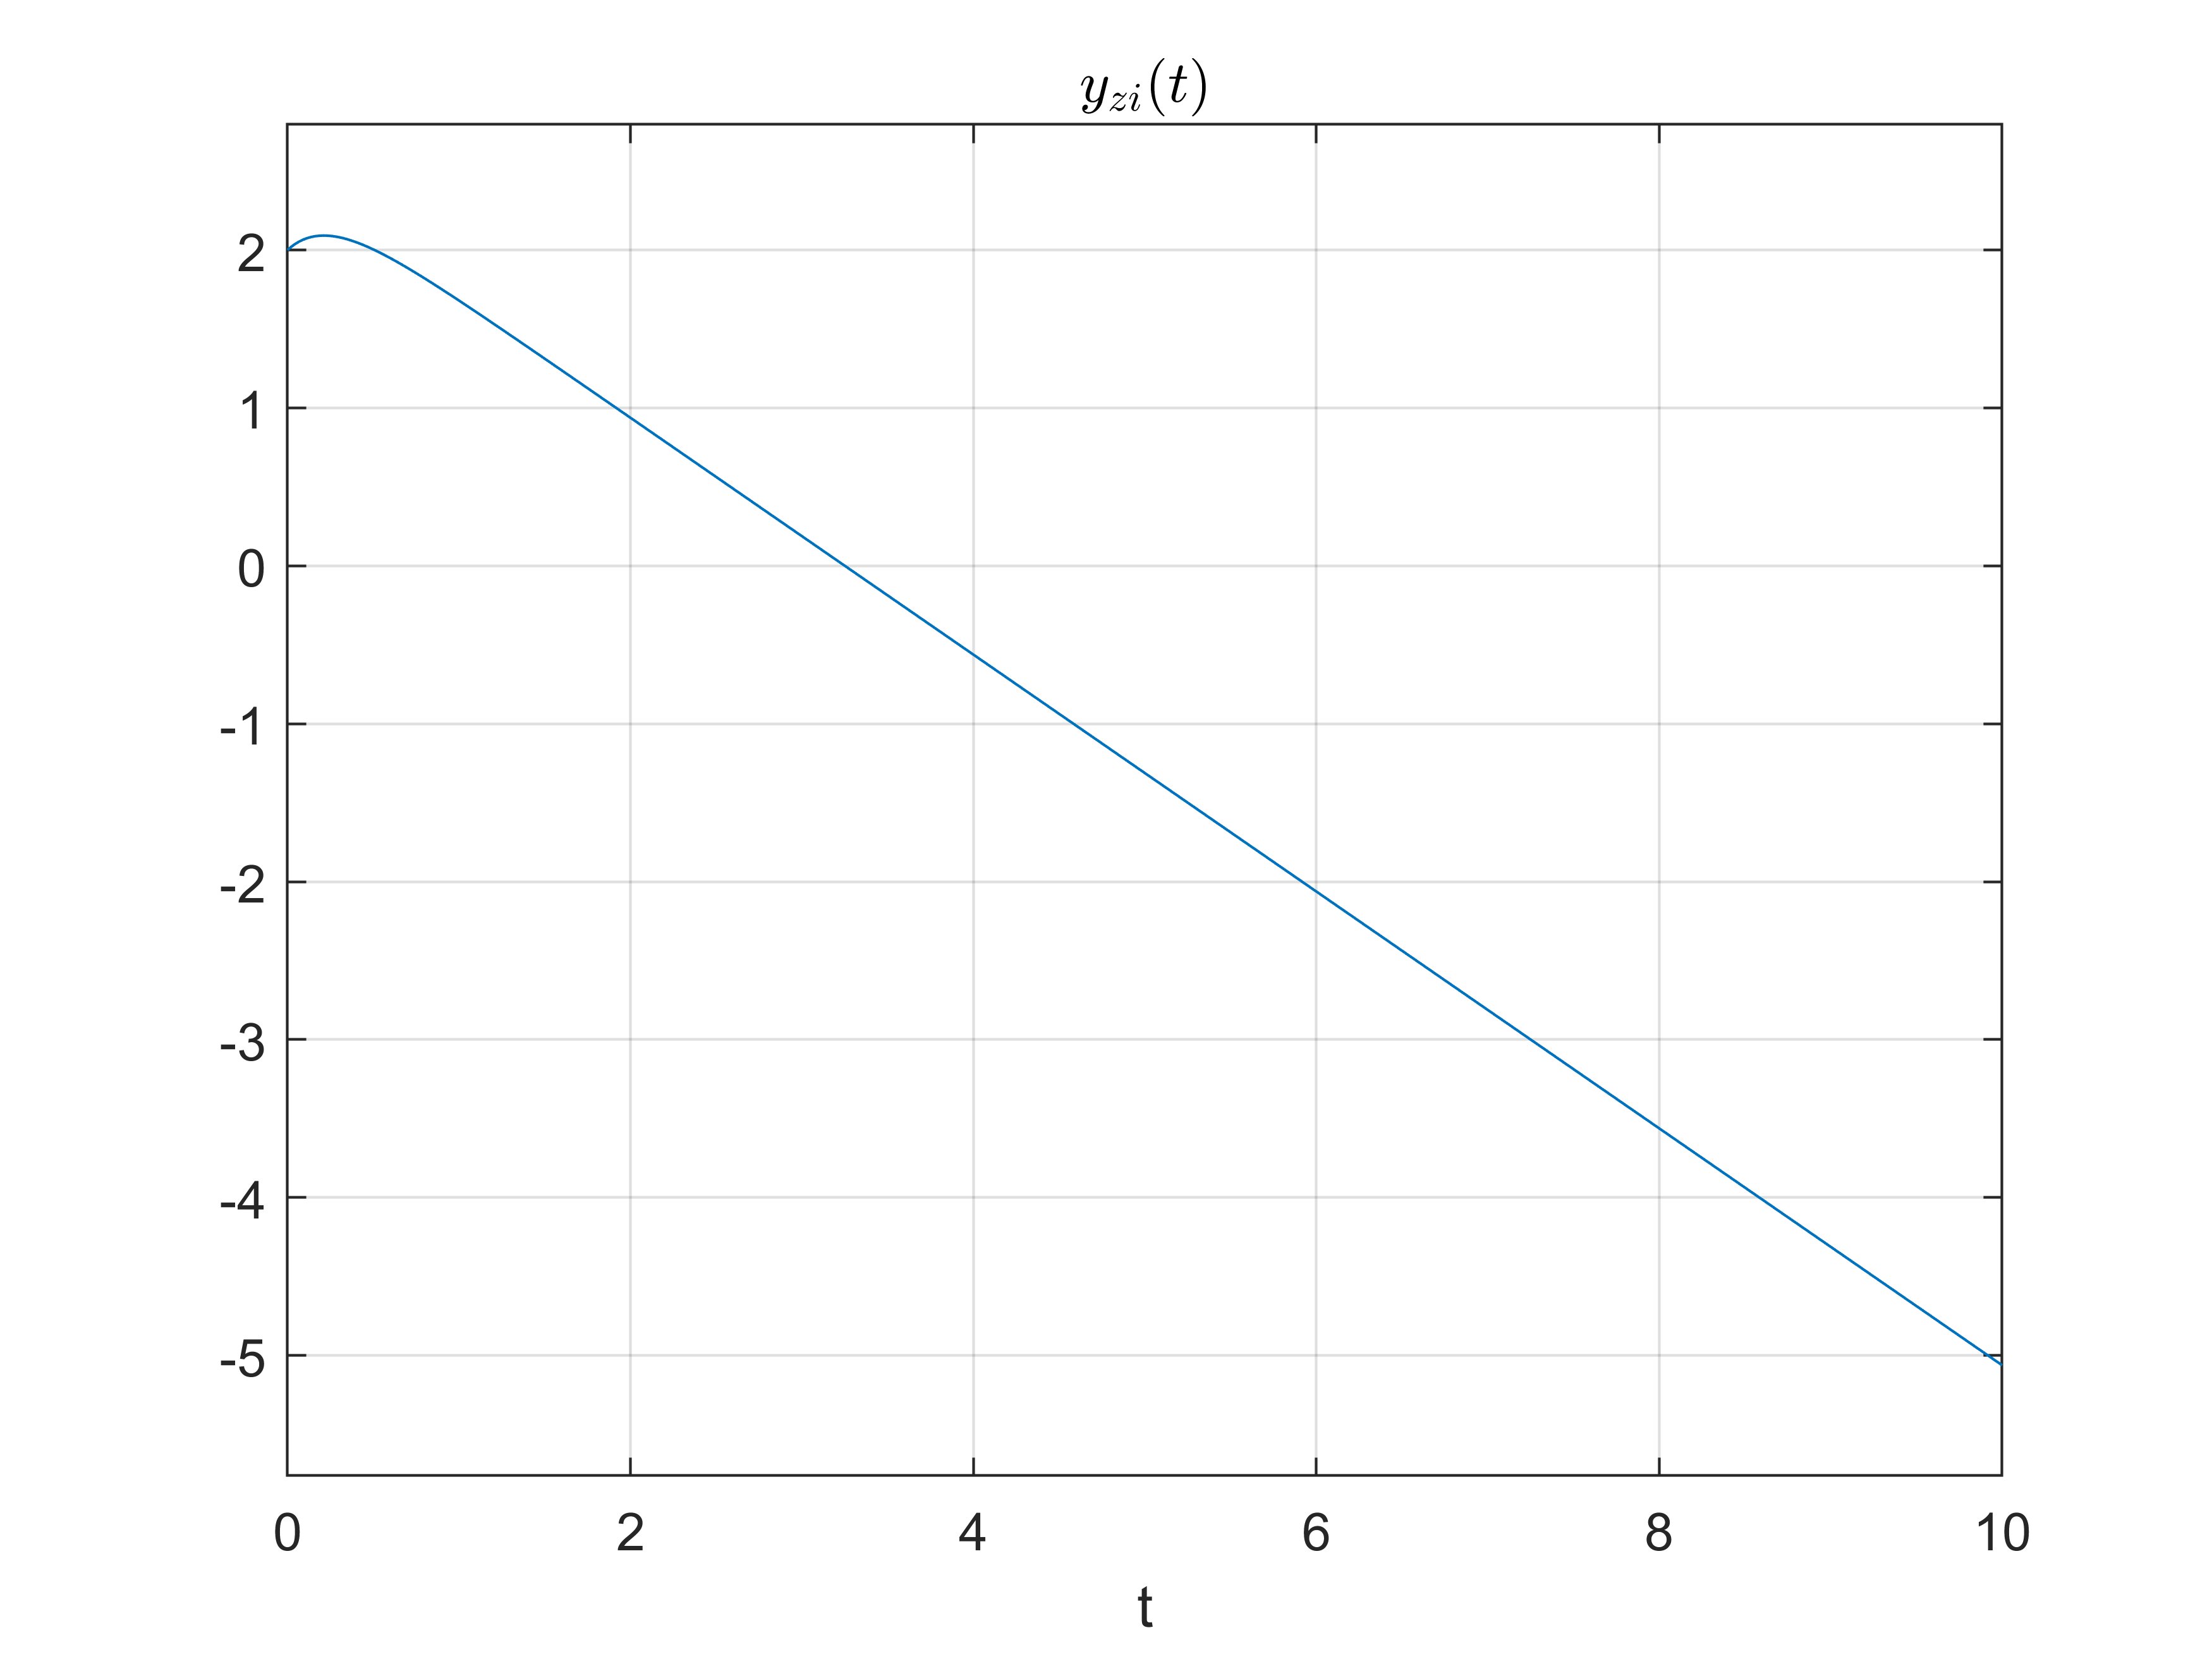
\includegraphics[scale=1]{符号法/2-zi.png}\\
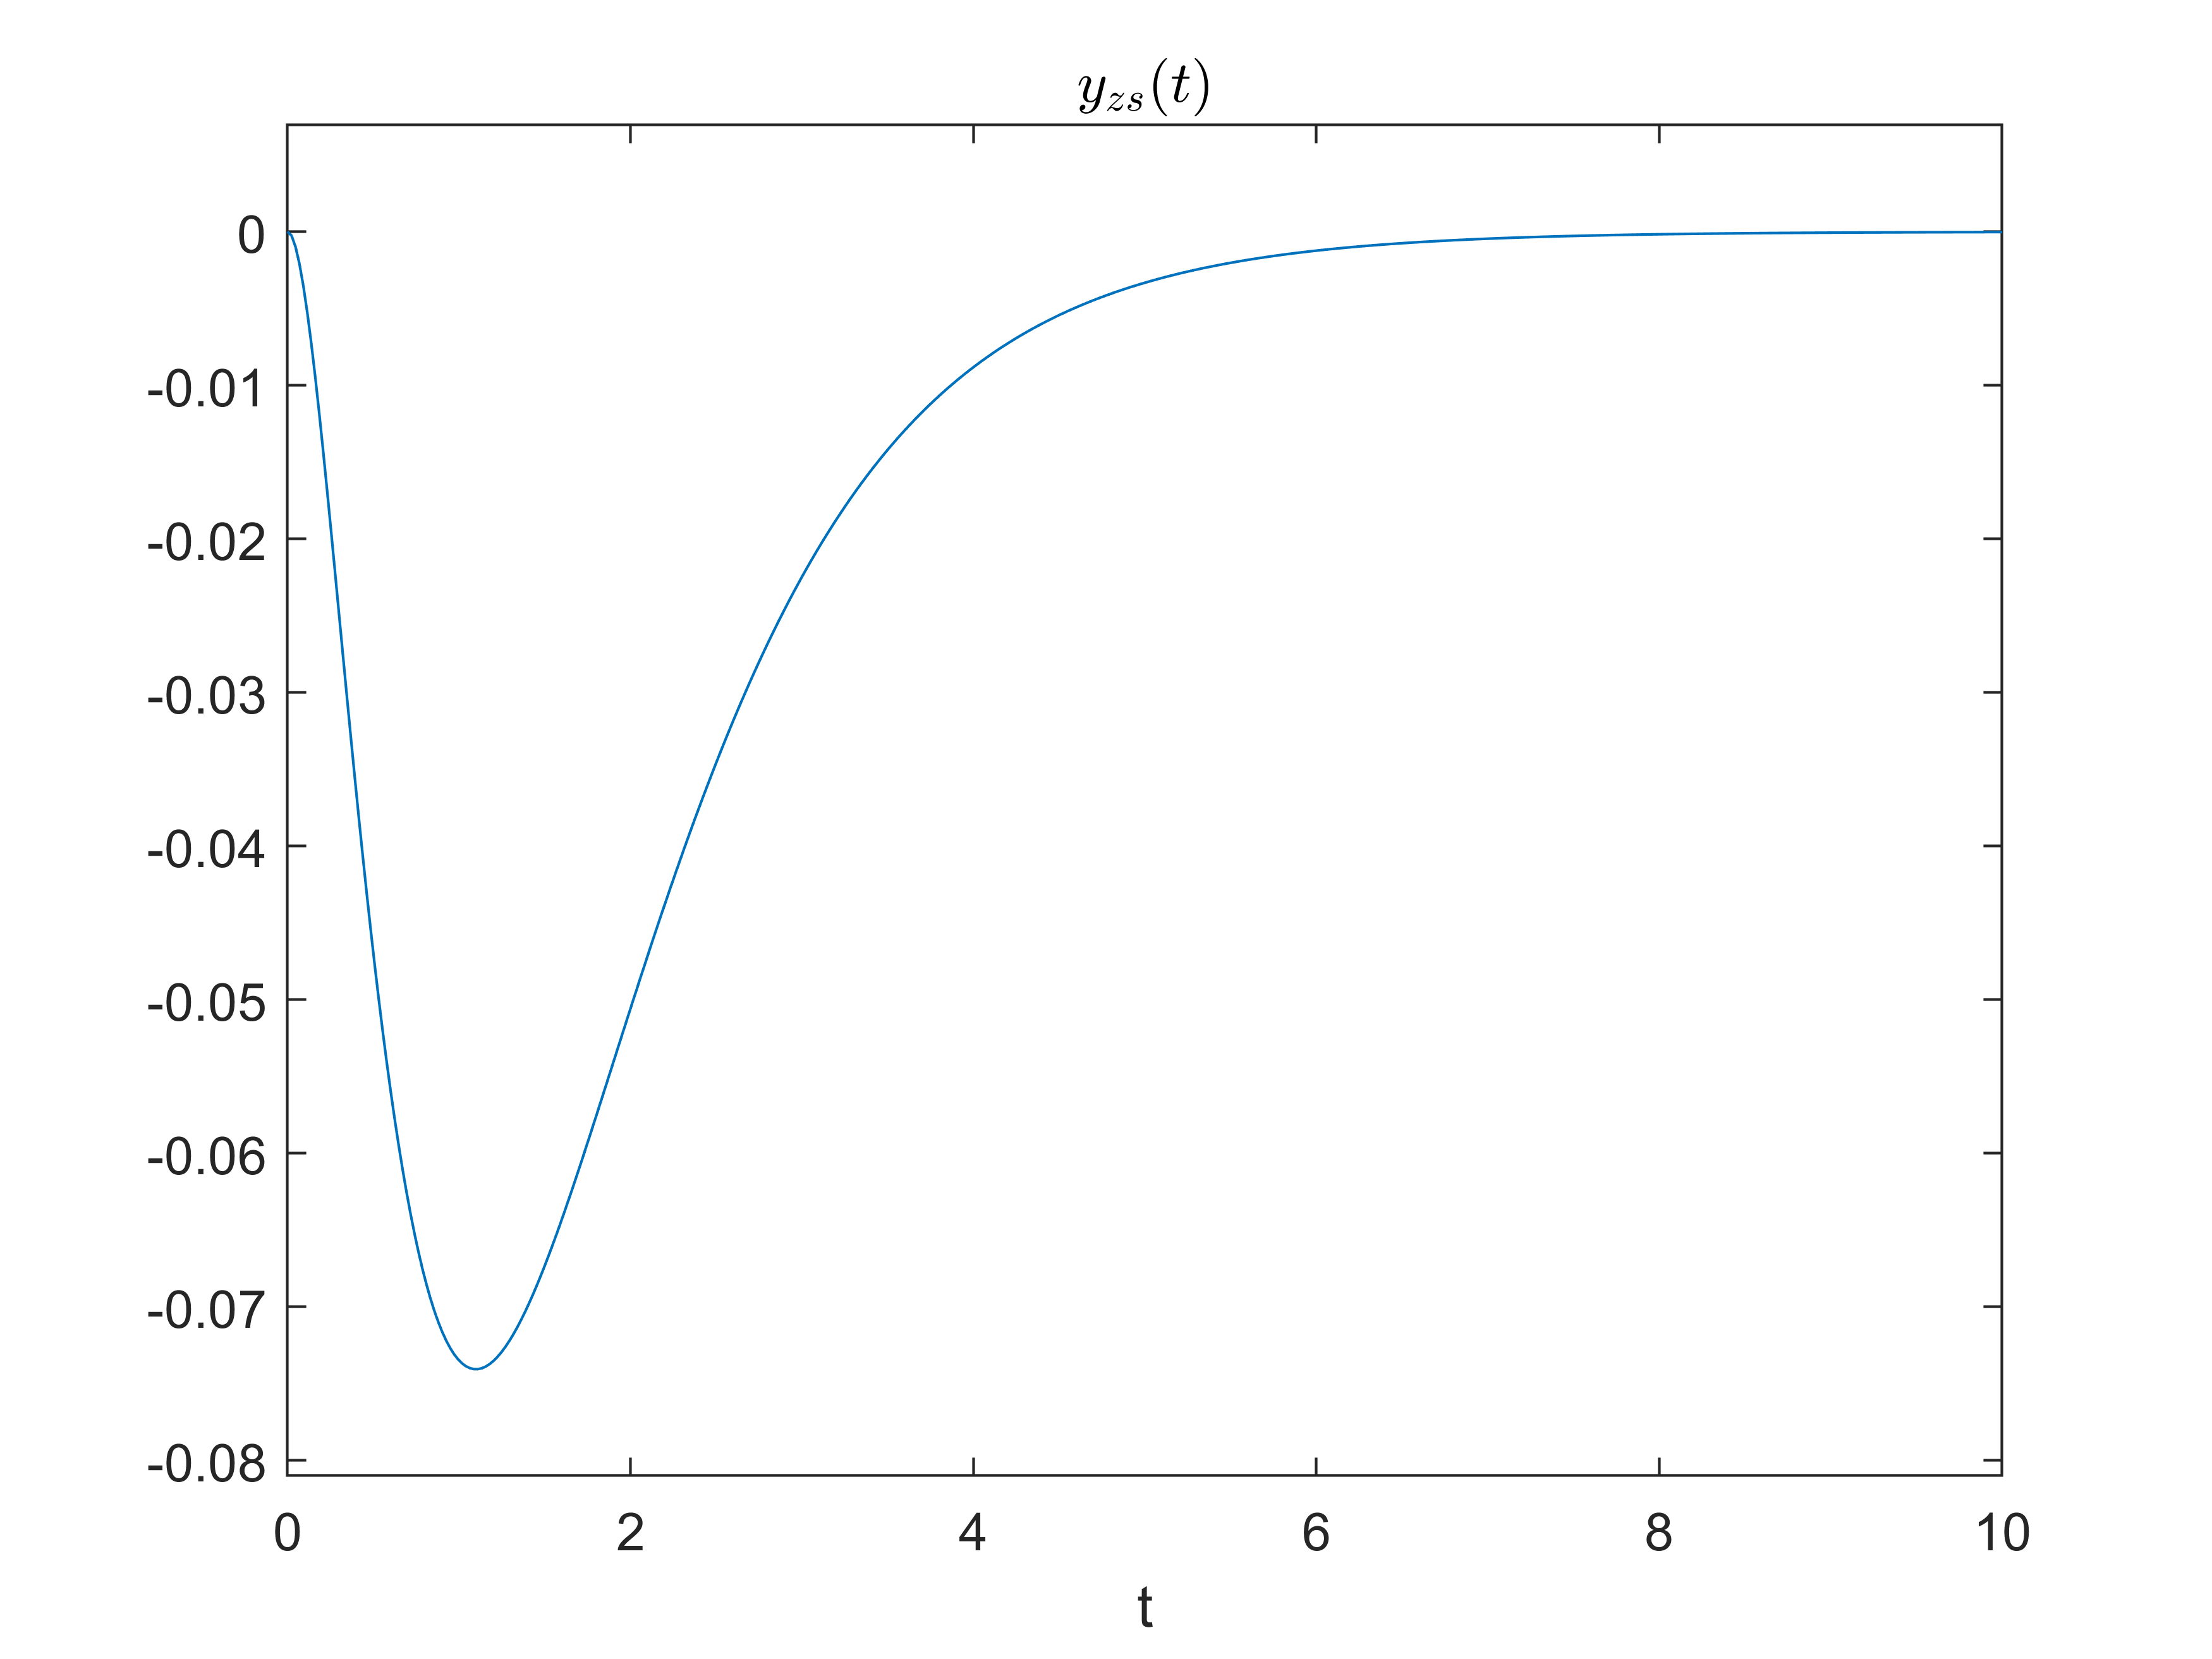
\includegraphics[scale=1]{符号法/2-zs.png}\\
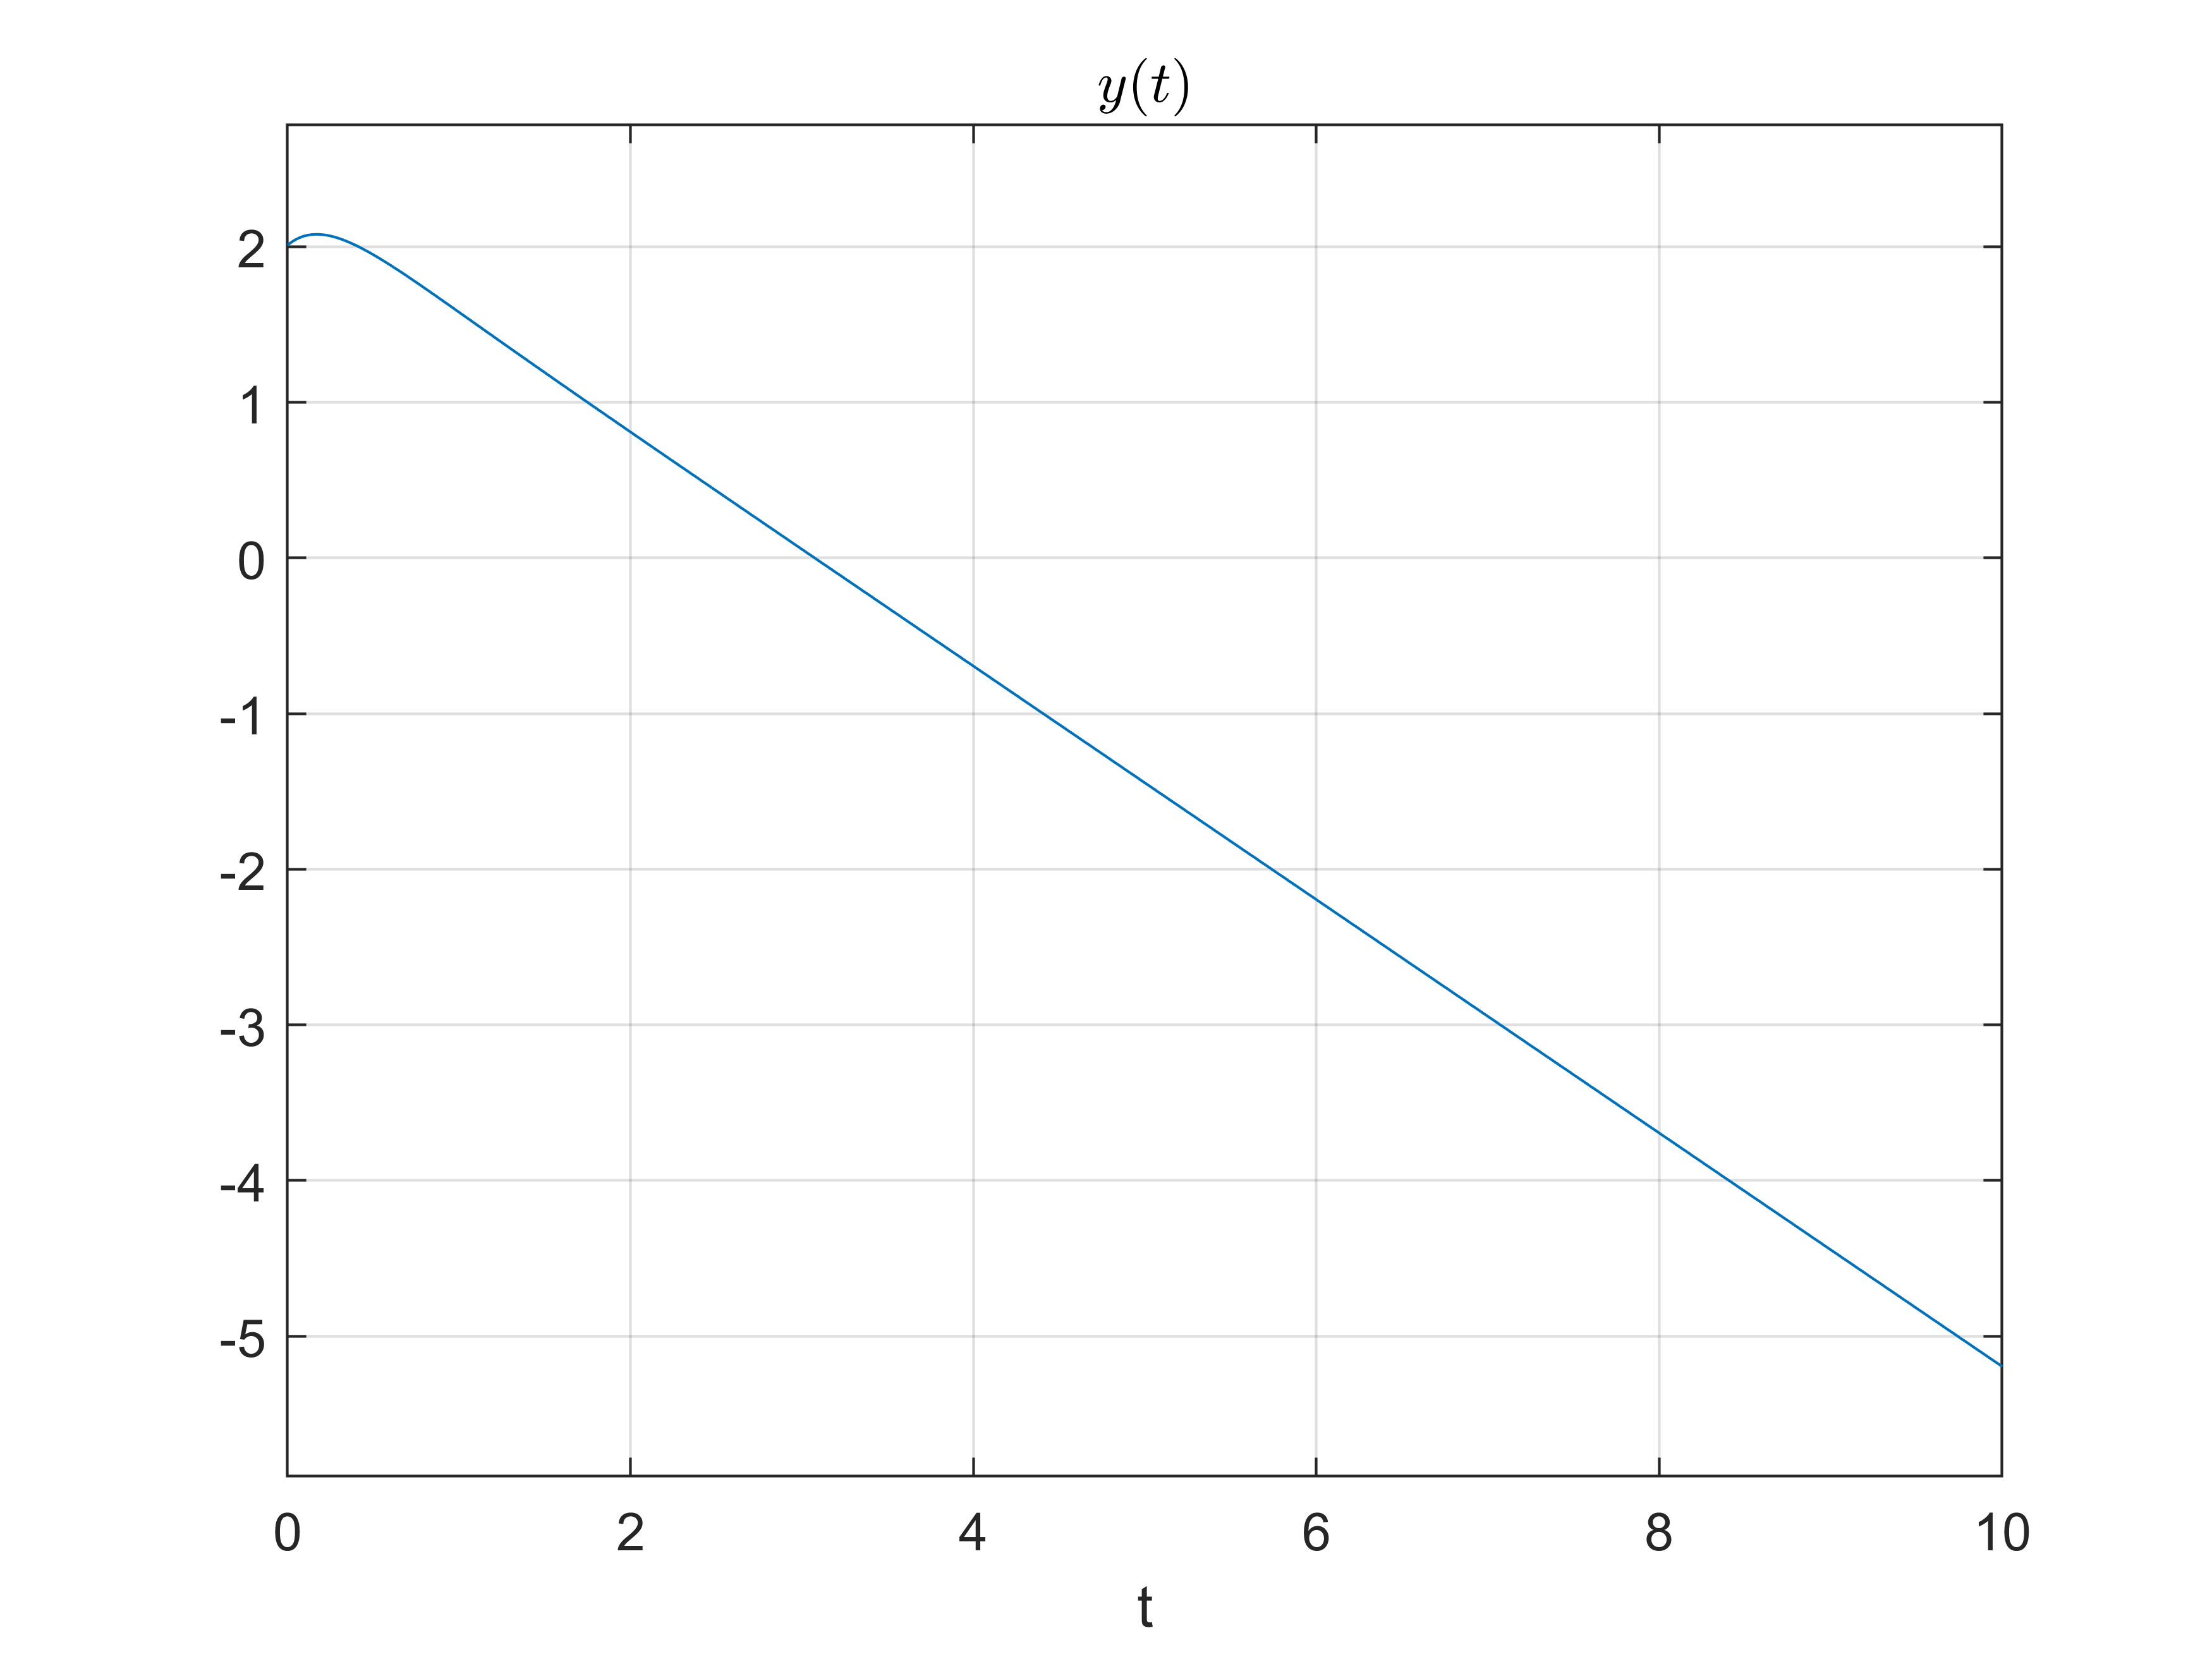
\includegraphics[scale=1]{符号法/2-all.png}
\section{Problem 3}
\subsection{Description}
Differential equations and excitation signals for known systems, zero-state response (with symbolism, numerical method, convolution integral method)
$$
\begin{aligned}
y''(t)+4y'(t)+3y(t)=f'(t)+2f(t),f(t)=e^{-2t}u(t)\\
y(0)=2,y'(0)=1
\end{aligned}
$$
Numberical method:\\
\begin{lstlisting}
	clear all;
	a=[1 4 3];
	b=[0 1 2];
	t=0:0.001:10;
	x=heaviside(t).*exp(-2*t);
	rc=[1,2];
	sys=tf(b,a)
	[A,B,C,D]=tf2ss(b,a)
	subplot(3,1,1),initial(A,B,C,D,rc,t) %零输入响应
	subplot(3,1,2),lsim(b,a,x,t)         %零状态响应
	subplot(3,1,3),lsim(A,B,C,D,x,t,rc)  %全响应,只能用状态系数来表示系统
\end{lstlisting}
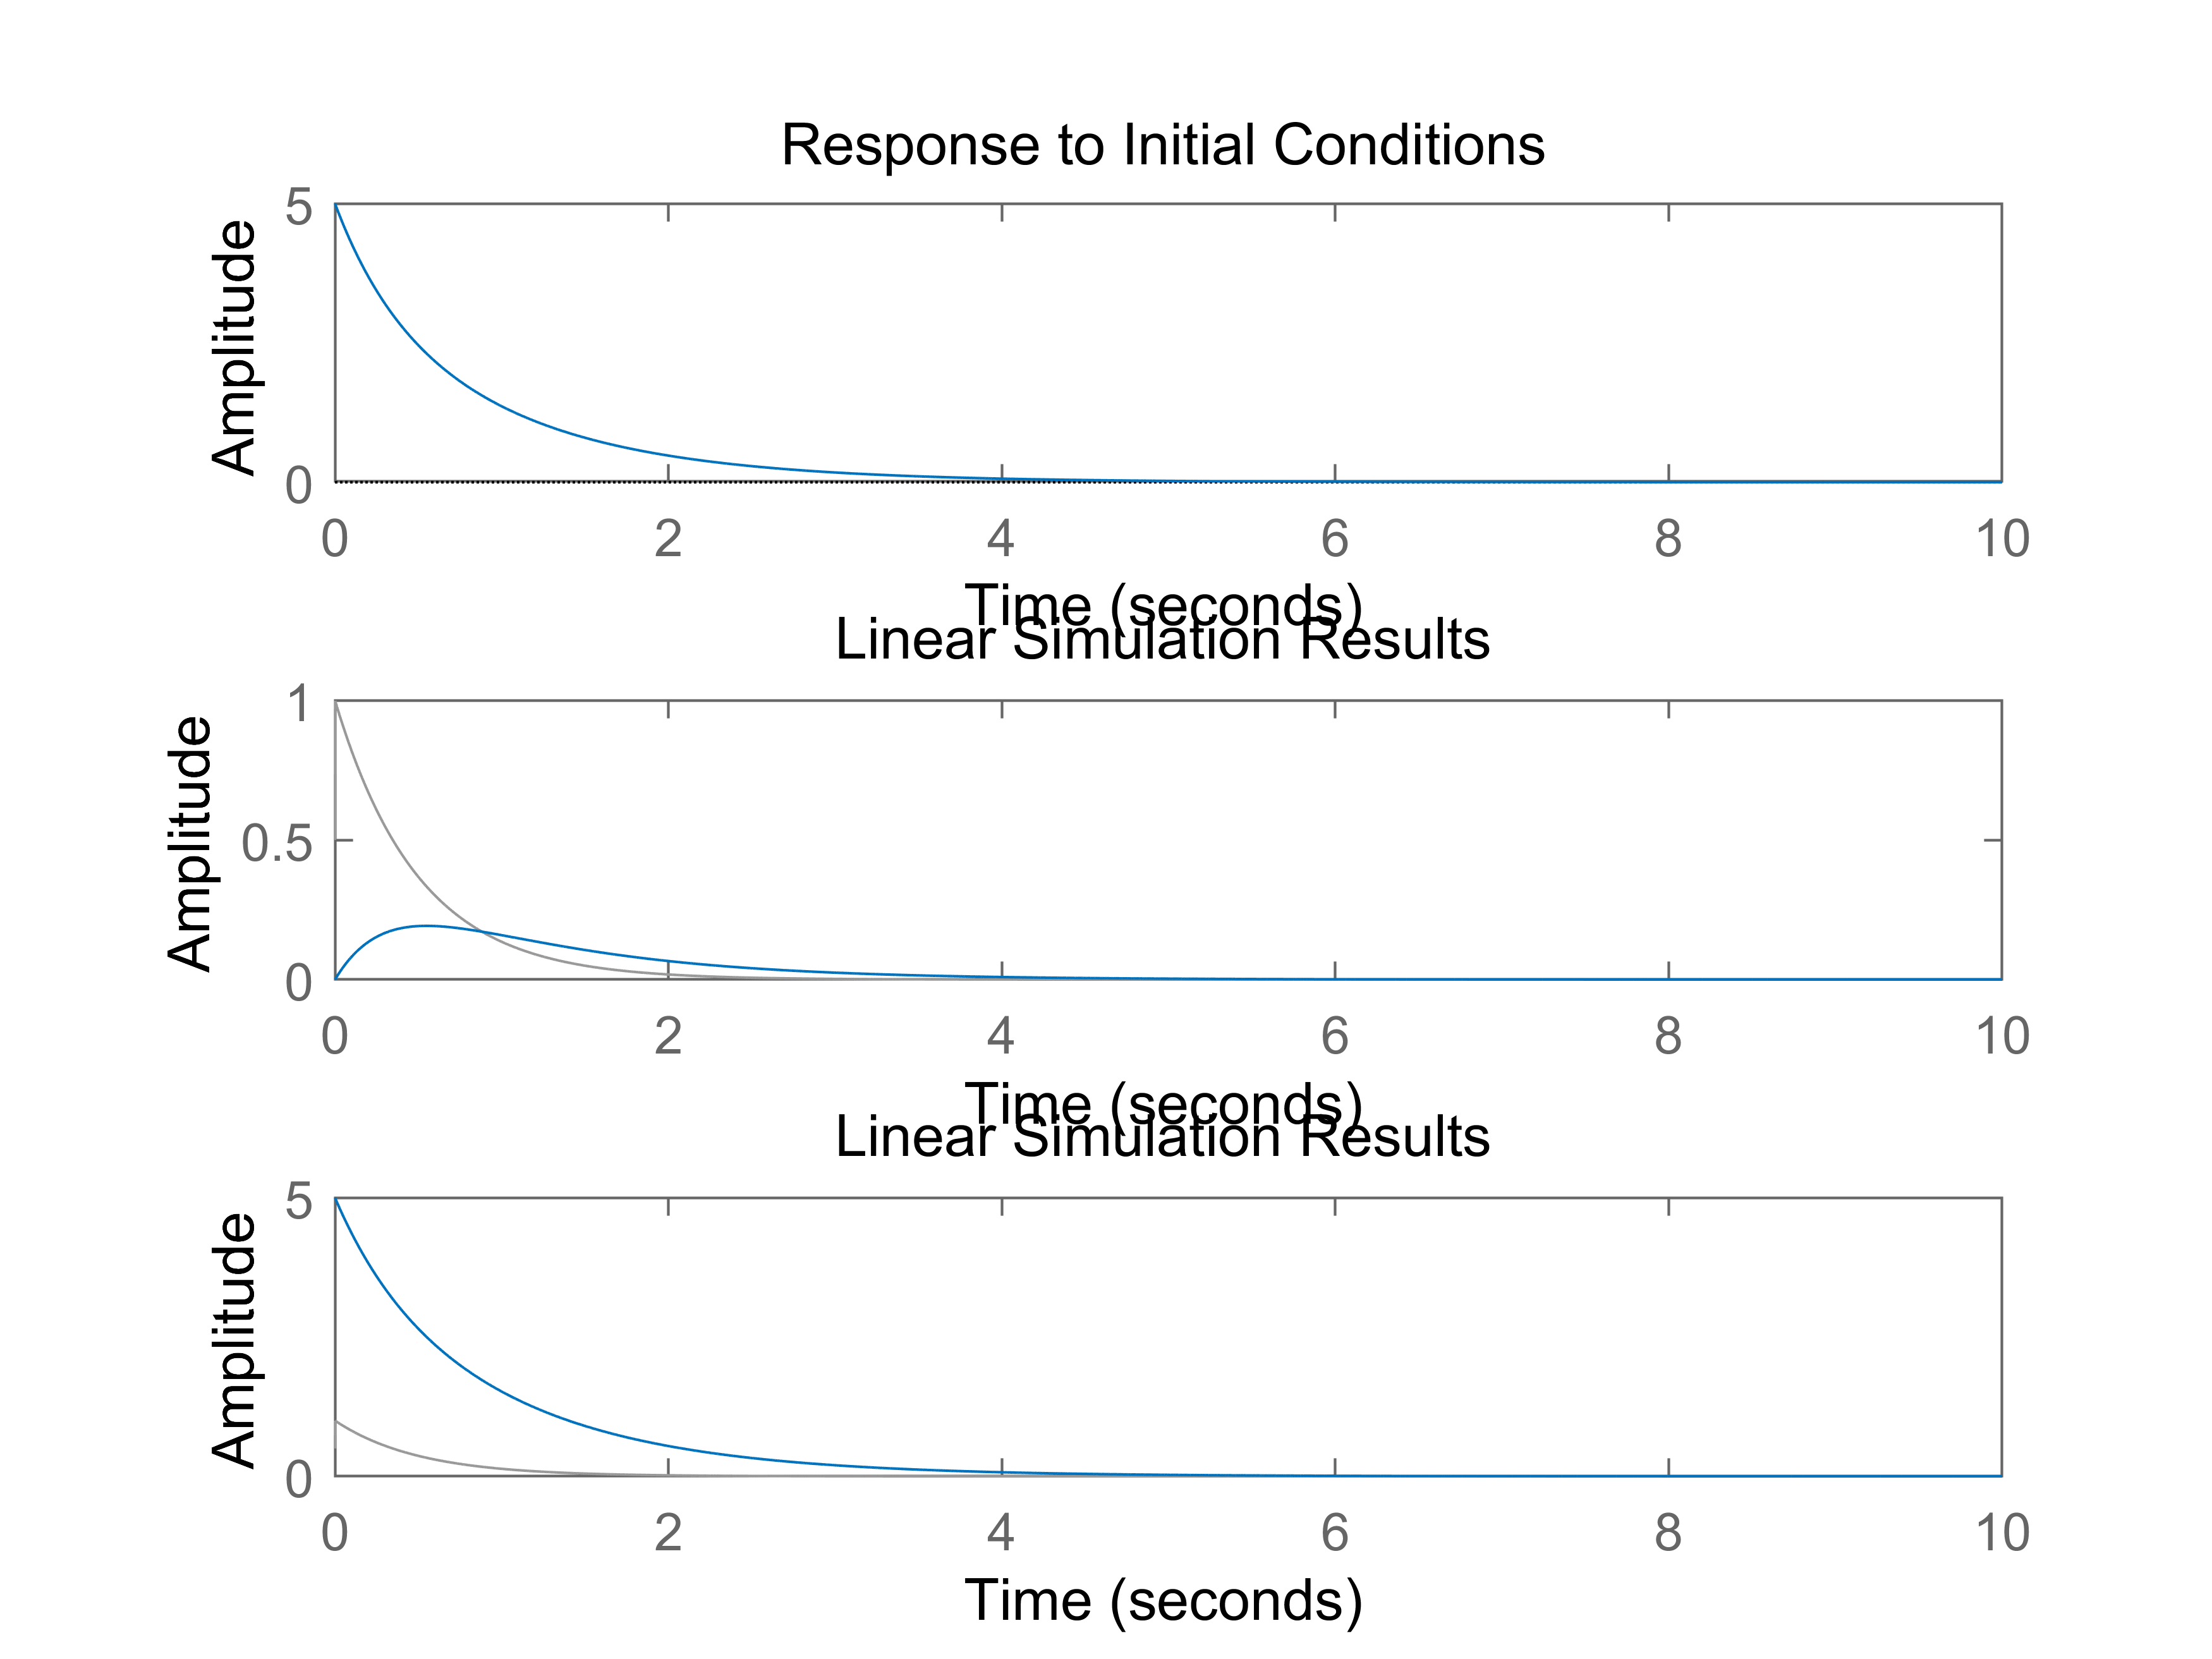
\includegraphics[scale=1]{数值3.png}
Symbolic method:\\
\begin{lstlisting}
	% 3
	% 零状态
	clear all 
	eq1 ='D2y+4*Dy+3*y=Dx+2*x' ;
	eq2 = 'x=heaviside(t)*exp(-2*t)' ;
	cond = 'y(-0.01)=0,Dy(-0.01)=0,D2y(-0.01)=0';
	ans1 = dsolve( eq1,eq2,cond); 
	simplify(ans1.y);
	ezplot(ans1.y,[0:0.01:10]) ;
	title('$y_{zs}(t)$','Interpreter','Latex');
	
	%3
	clear all;
	%零输入响应
	eq1_1 ='D2y+4*Dy+3=0' ;
	cond_1 ='y(0)=2,Dy(0)=1';
	yzi = dsolve(eq1_1,cond_1);
	ezplot(yzi,[0:0.01:10])
	hold on;
	title('$y_{zi}(t)$','Interpreter','Latex');
	grid on;
	
	%3
	clear all;
	%全响应响应
	eq1_1 ='D2y+4*Dy+3=Dx+2*x';
	eq2 = 'x=heaviside(t)*exp(-2*t)';
	cond_1 ='y(-0.01)=2,Dy(-0.01)=1';
	ans = dsolve(eq1_1,eq2,cond_1);
	ezplot(ans.y,[0:0.01:10])
	title('$y(t)$','Interpreter','Latex');
	hold on;
	grid on;
\end{lstlisting}
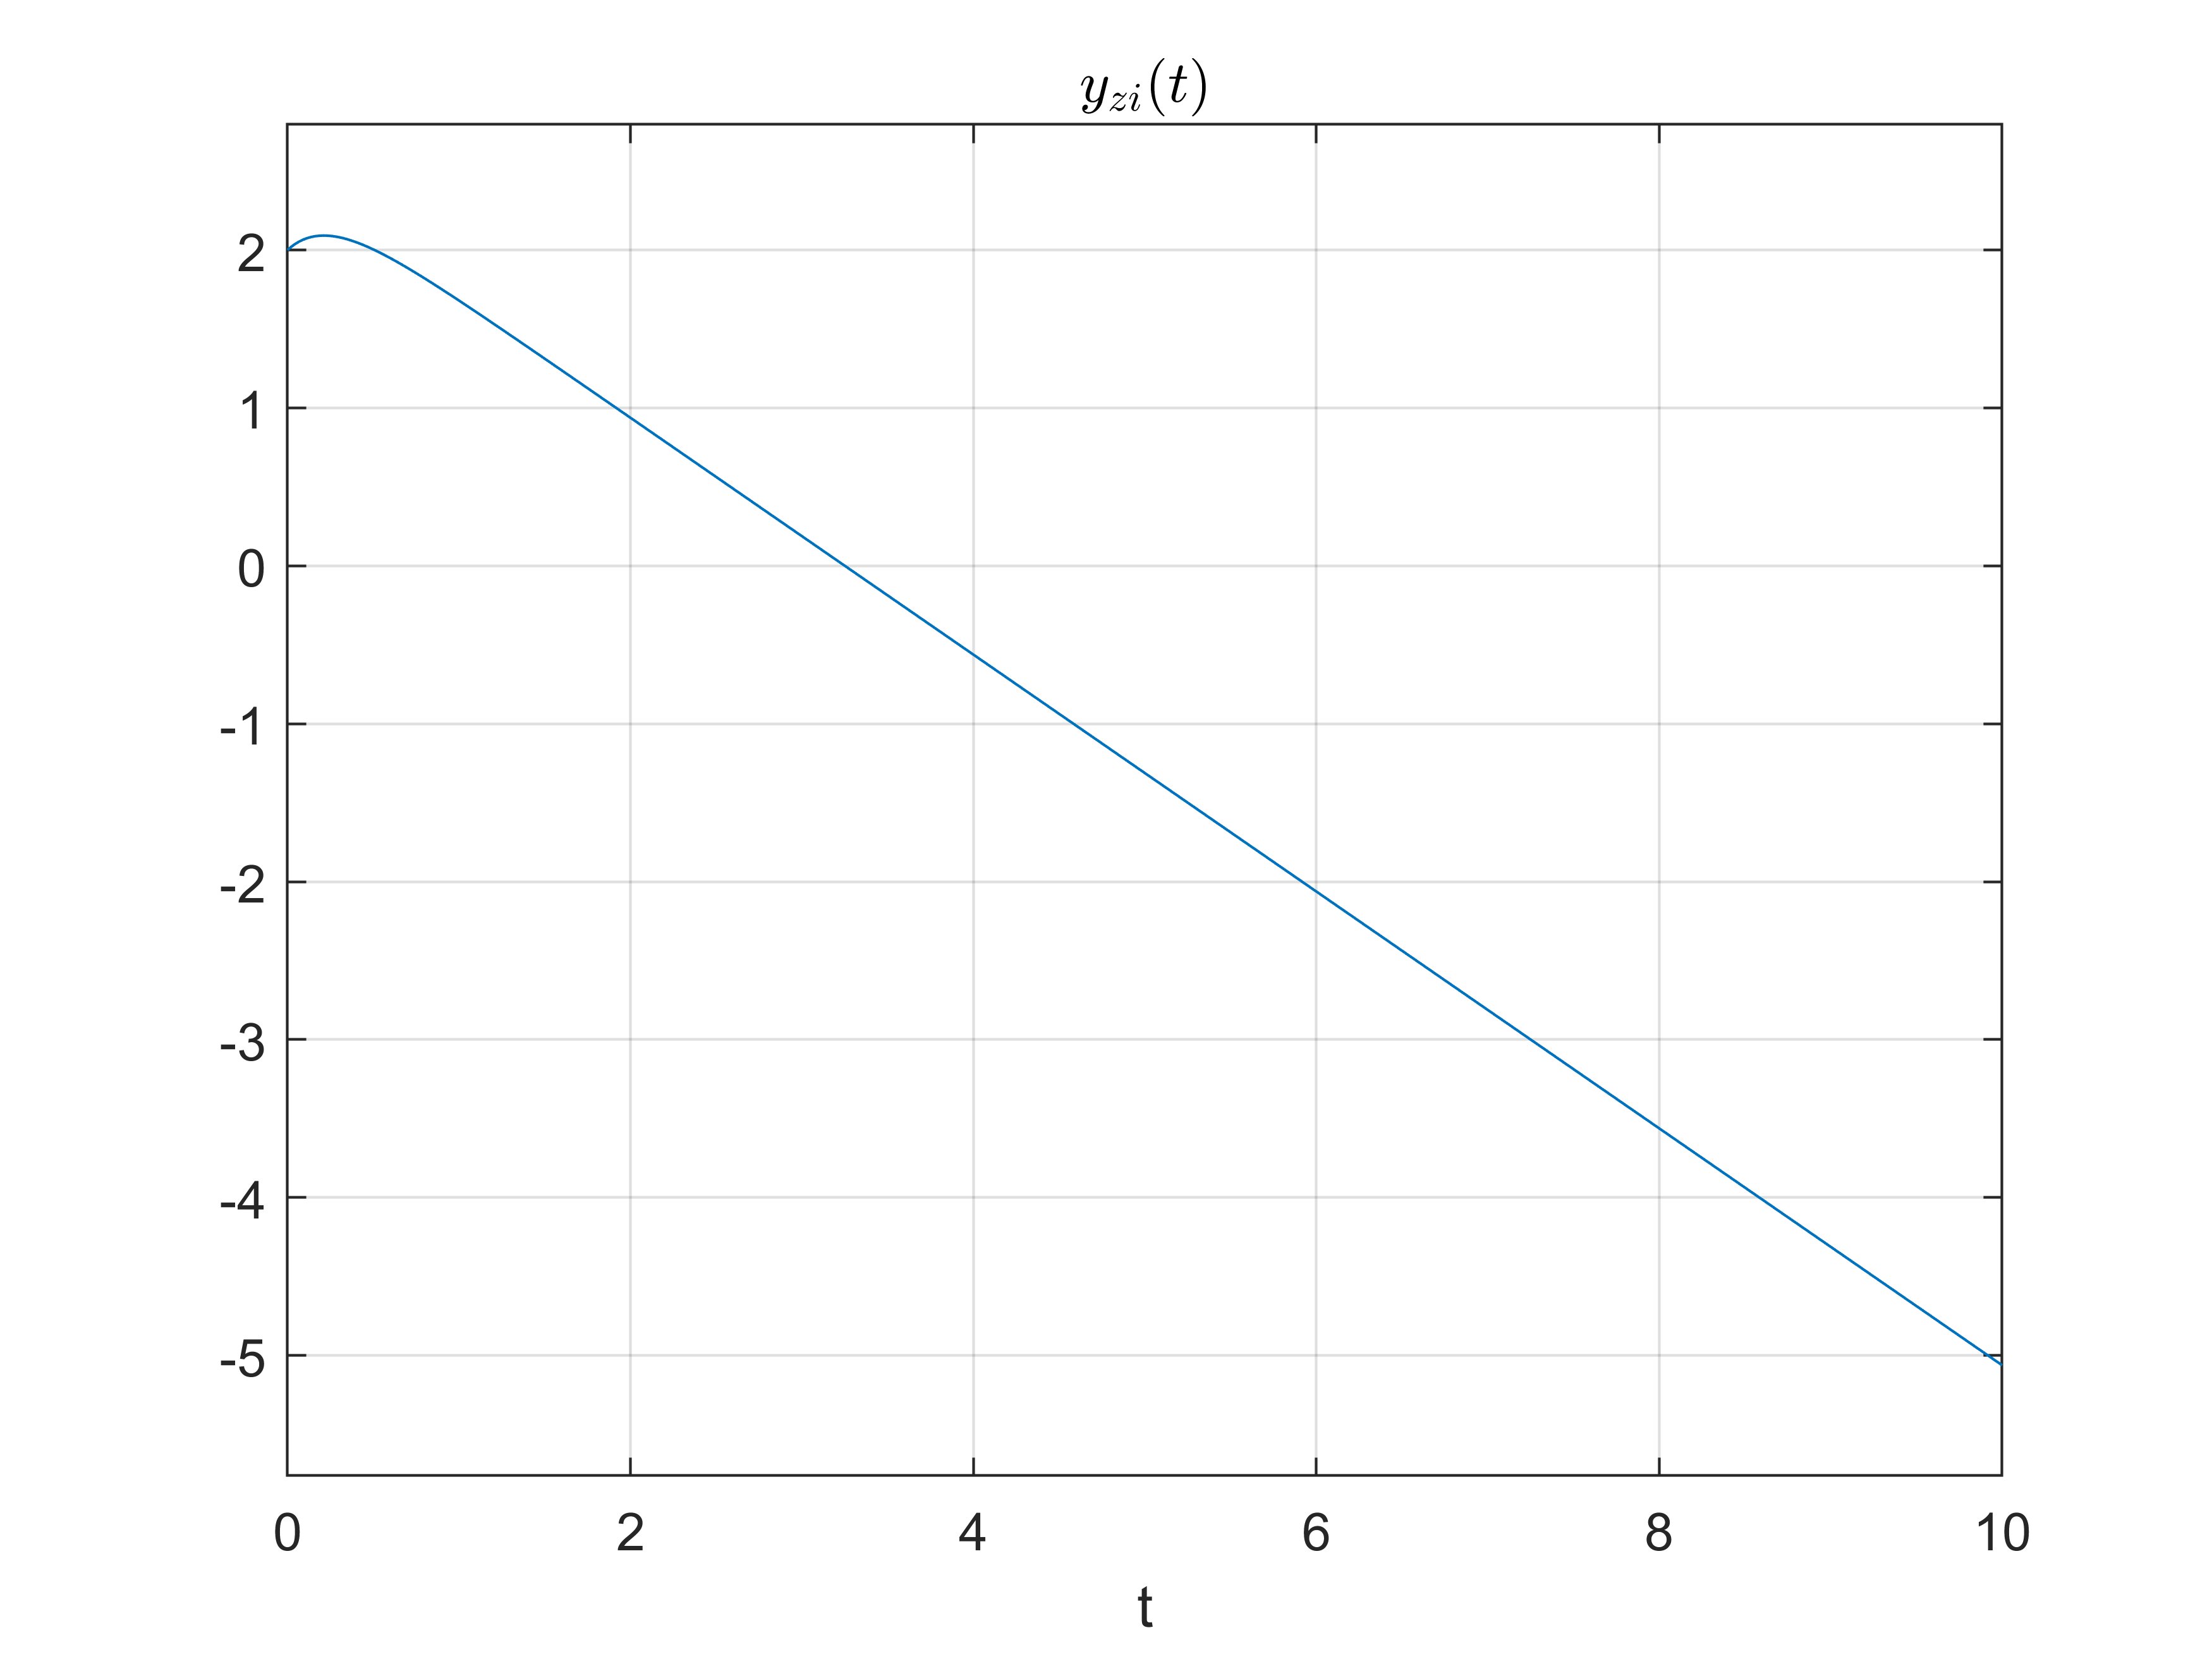
\includegraphics[]{符号法/3-zi.png}\\
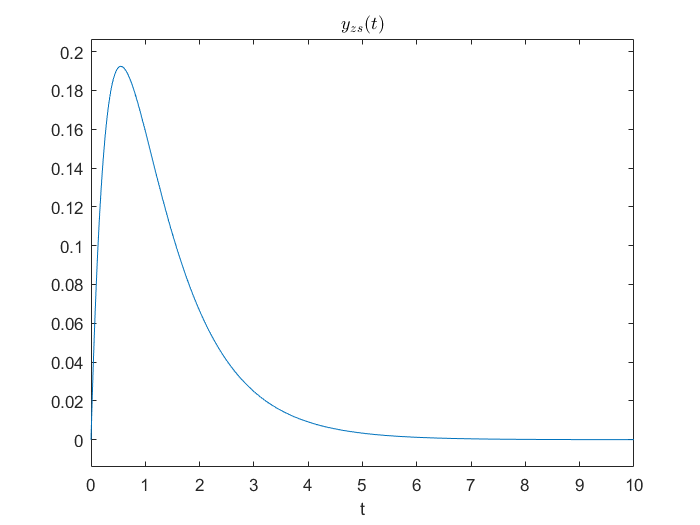
\includegraphics[]{符号法/3-zs.png}\\
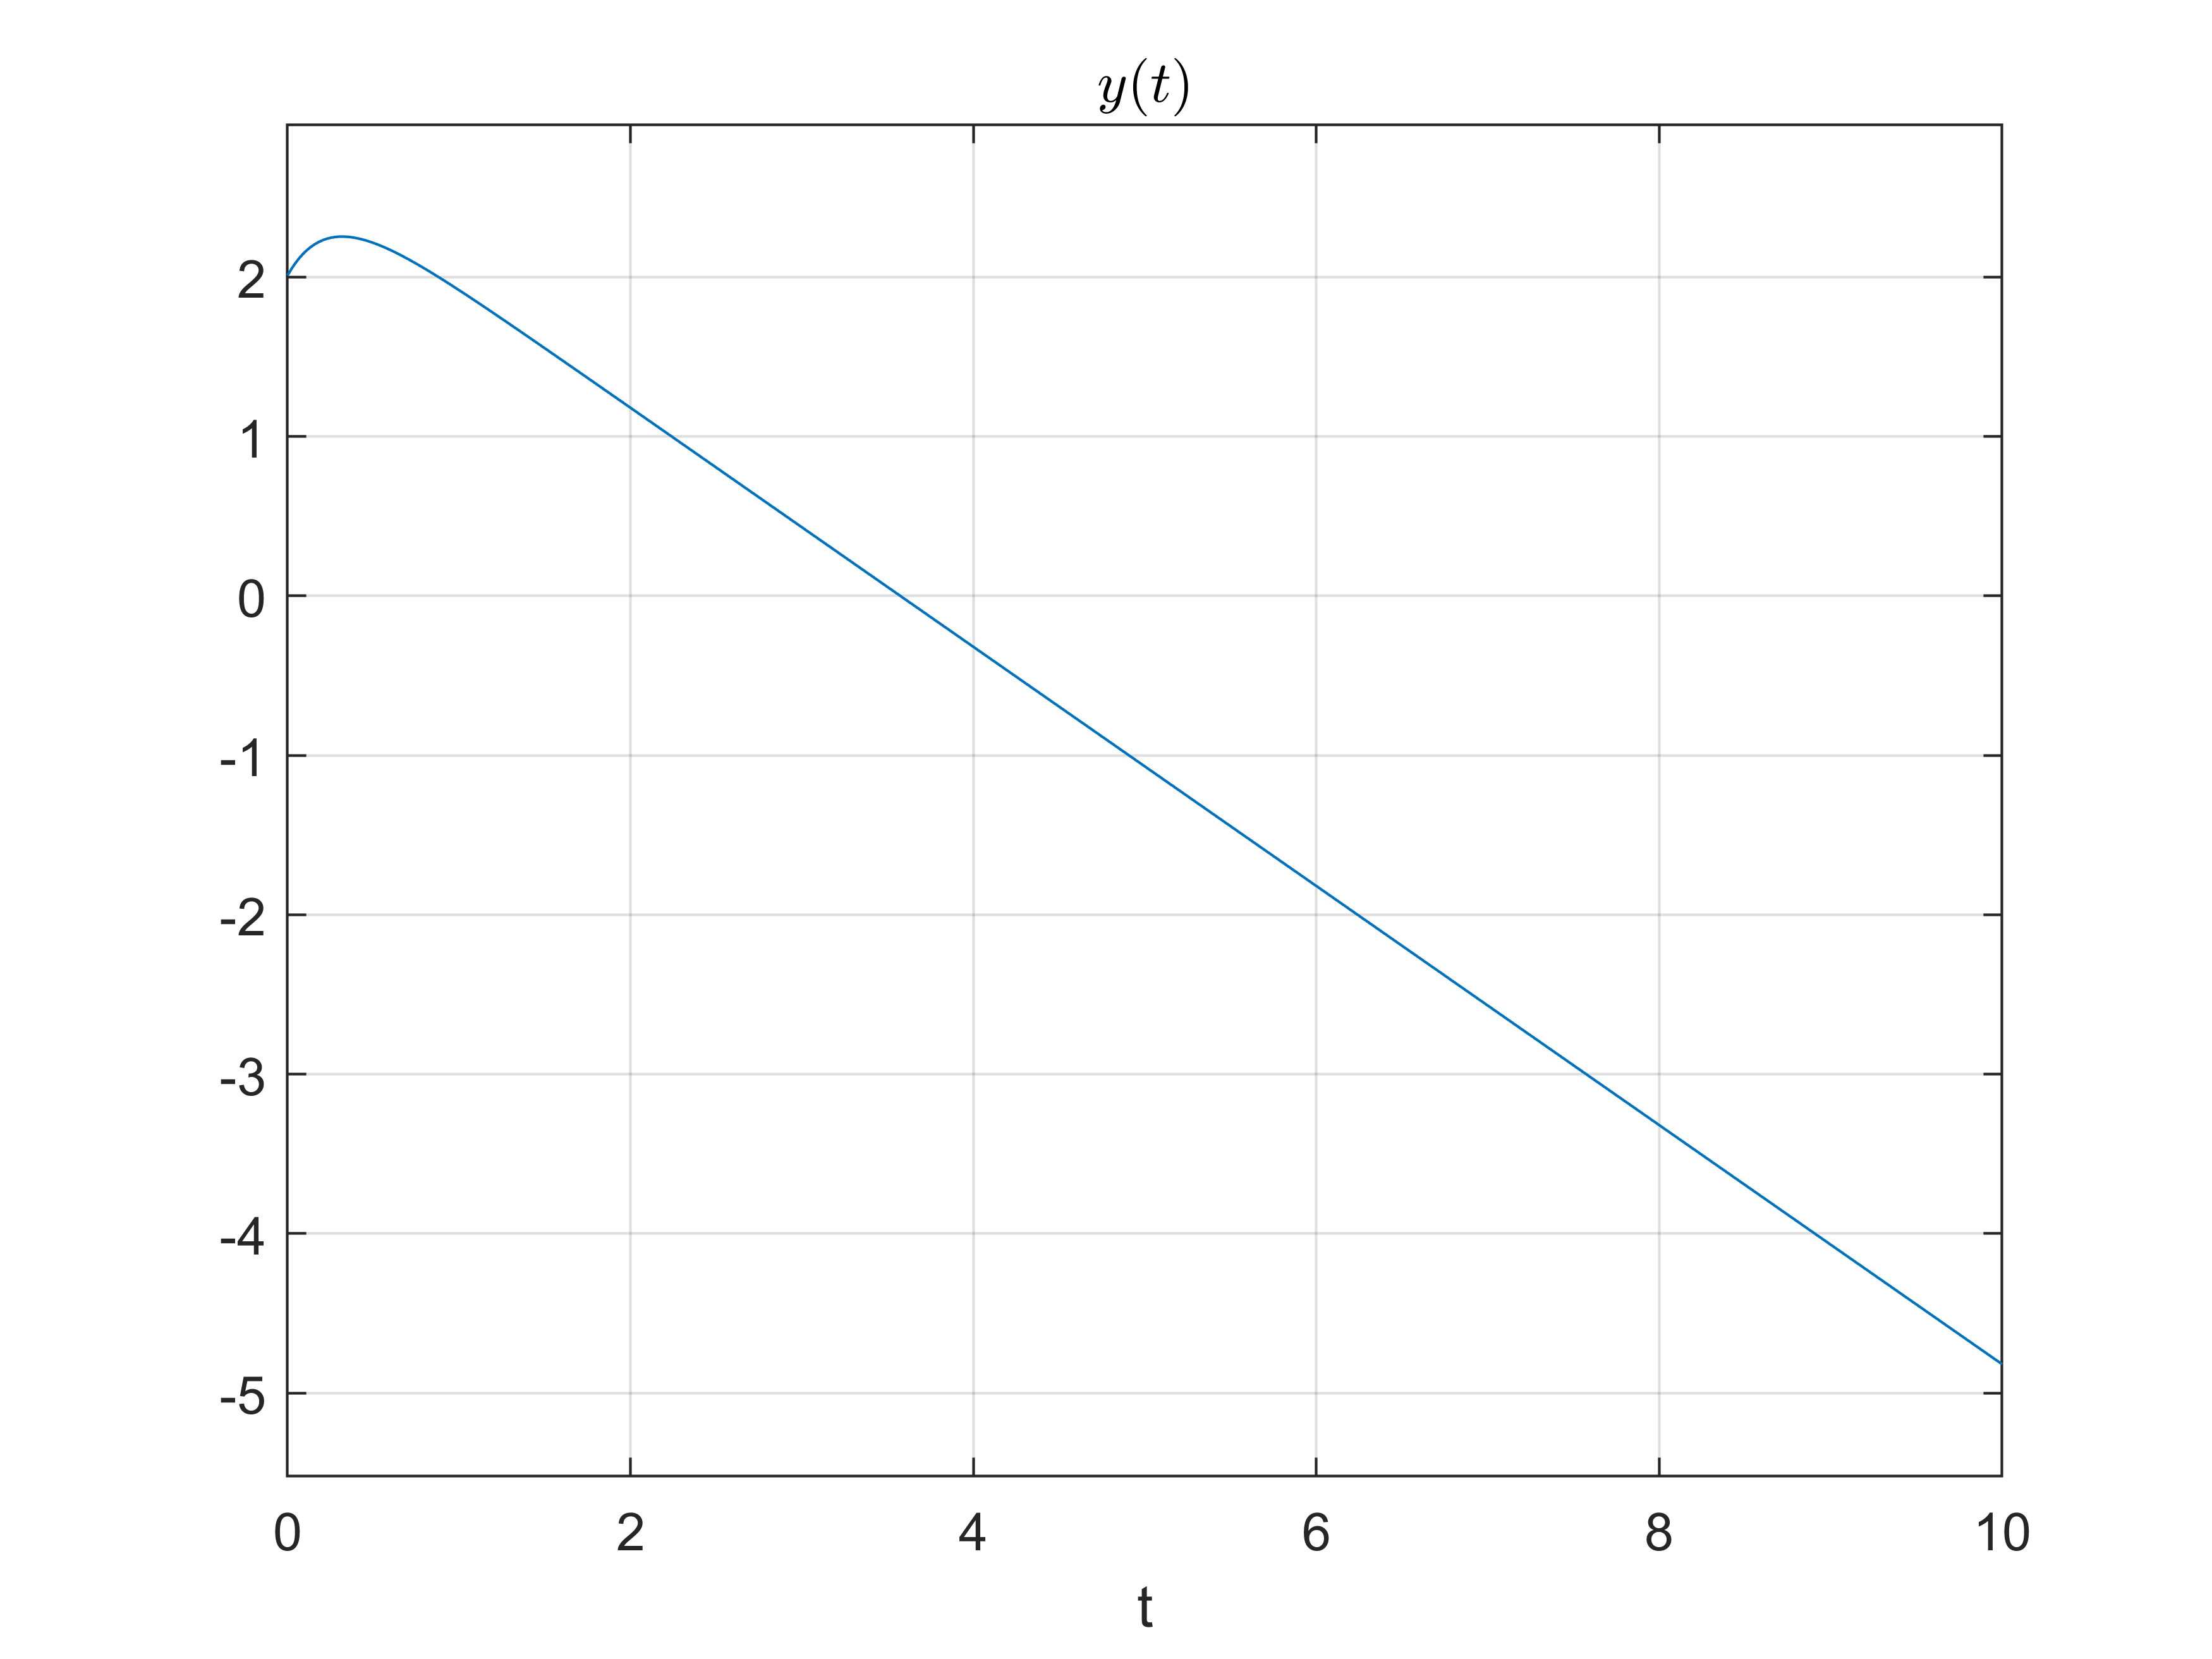
\includegraphics[]{符号法/3-all.png}\\
\section{Problem 4}
\subsection{Description}
Differential equations for known systems, unit impulse response and unit step response
$$
\begin{aligned}
y''(t)+3y'(t)+2y(t)=f(t)\\
y''(t)+2y'(t)+2y(t)=f'(t)
\end{aligned}
$$
Symbolic method:\\
\begin{lstlisting}
	4-1
	clear all
	eq1 ='D2y+3*Dy+2*y=heaviside(t)' ;
	cond = 'y(-0.01)=0,Dy(-0.01)=0,D2y(-0.01)=0';
	ans1 = dsolve(eq1,cond); 
	simplify(ans1);
	ezplot(ans1,[0:0.01:10]);
	hold on;
	grid on;
	title('y(t)')
	
	% 4-2
	clear all
	eq1 ='D2y+2*Dy+2*y=dirac(t)';
	cond = 'y(0)=0,Dy(0)=0';
	ans1 = dsolve(eq1,cond);
	ezplot(ans1);
	grid on;
	title('y(t)')
\end{lstlisting}
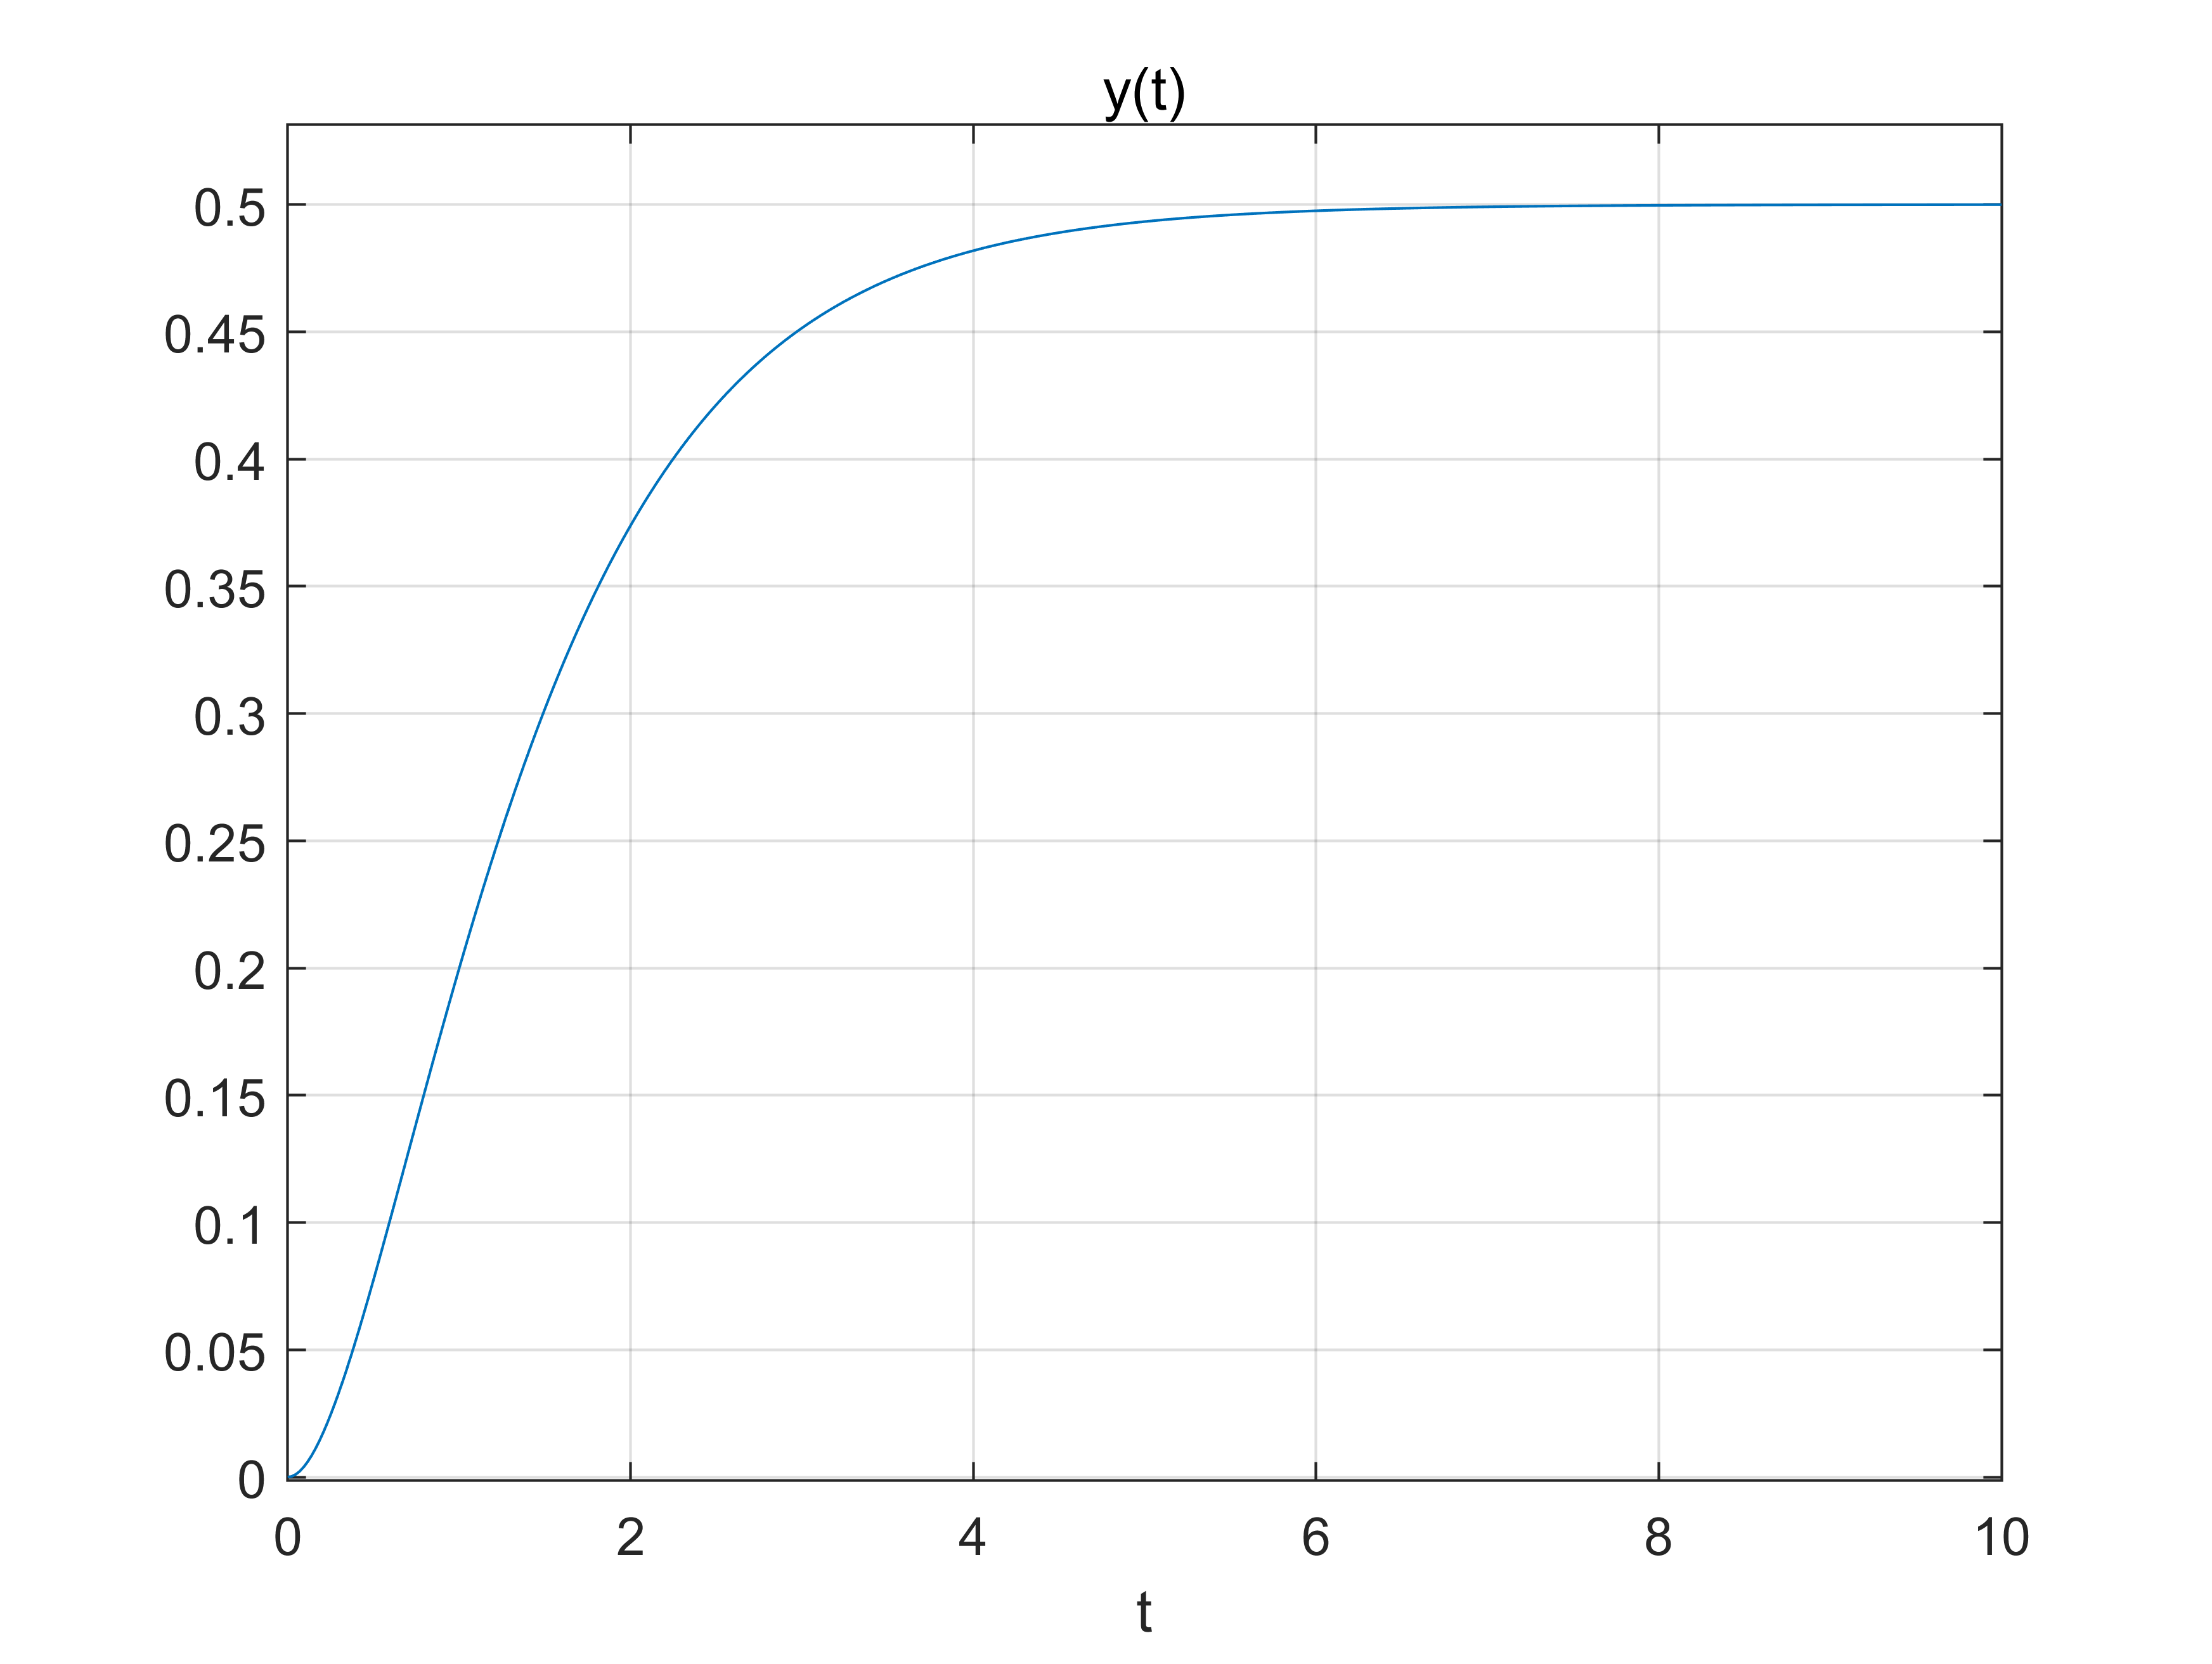
\includegraphics[scale=1]{符号法/4-1.png}\\
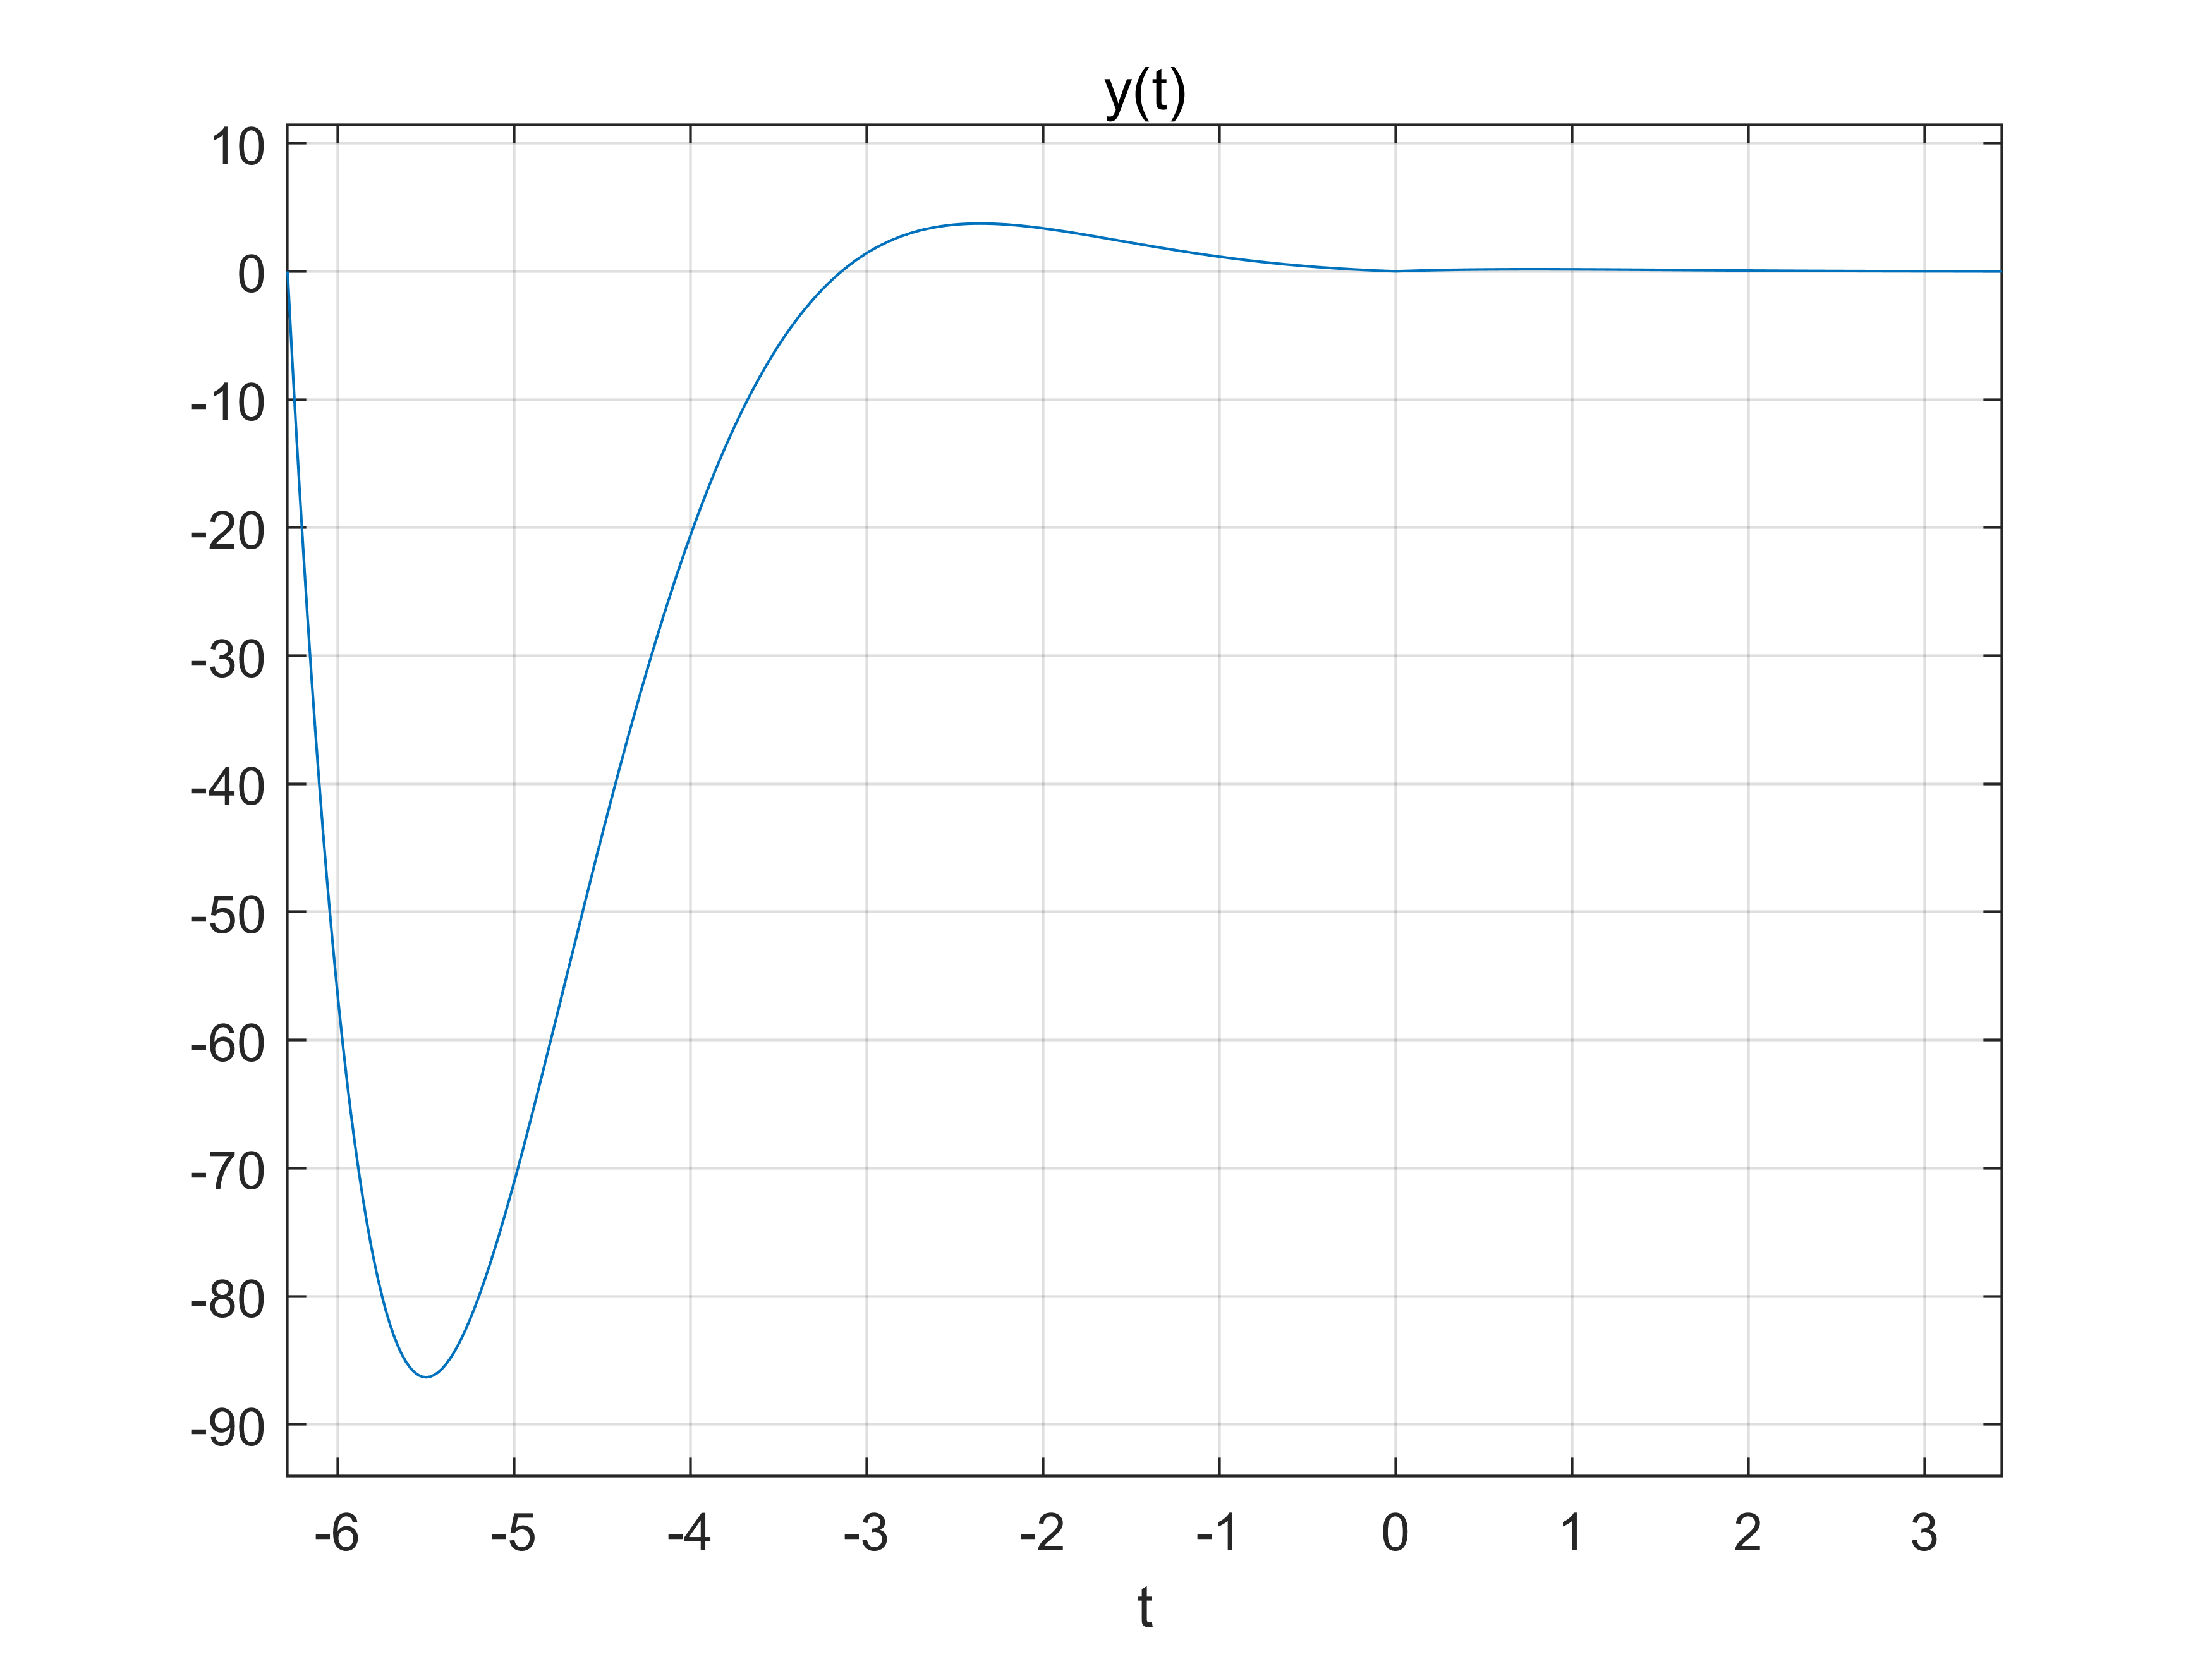
\includegraphics[scale=1]{符号法/4-2.png}\\
\end{document}